\documentclass[12pt,a4paper]{report}
\usepackage[utf8]{inputenc}
\usepackage[T1]{fontenc}
\usepackage[french,english]{babel}
\usepackage{geometry}
\geometry{margin=2.5cm, top=3cm}
\setlength{\headheight}{14.5pt}
\usepackage{graphicx}
\graphicspath{{../diagrams/presentation/exported/}{../diagrams/technical/exported/}}
\usepackage{hyperref}
\usepackage{listings}
\usepackage{xcolor}
\usepackage{booktabs}
\usepackage{longtable}
\usepackage{float}
\usepackage{fancyhdr}
\usepackage{titlesec}
\usepackage{tocloft}
\usepackage{enumitem}

% Colors
\definecolor{stblue}{RGB}{26,35,126}
\definecolor{codebg}{RGB}{245,245,245}
\definecolor{codeframe}{RGB}{200,200,200}

% Code listing style
\lstset{
  backgroundcolor=\color{codebg},
  frame=single,
  rulecolor=\color{codeframe},
  basicstyle=\ttfamily\small,
  breaklines=true,
  keywordstyle=\color{blue},
  commentstyle=\color{gray},
  stringstyle=\color{red!70!black},
}

% Headers
\pagestyle{fancy}
\fancyhf{}
\fancyhead[L]{\leftmark}
\fancyhead[R]{STM32Cube Preprocessing Pipeline}
\fancyfoot[C]{\thepage}

\hypersetup{
  colorlinks=true,
  linkcolor=stblue,
  urlcolor=blue!70!black,
  citecolor=stblue,
}

\title{
  \vspace{-2cm}
  %\includegraphics[width=4cm]{placeholder_st_logo.png}\\[1cm]
  \vspace{1cm}
  \textbf{\Huge STM32Cube GitHub Preprocessing Pipeline}\\[0.5cm]
  \textbf{\Large Technical Documentation}\\[0.3cm]
  \large Enterprise Reference Document\\[1cm]
  \normalsize Version 2.0 --- June 2026
}
\author{
  Abir Gharbi\\
  STMicroelectronics --- AI \& Digital Tools Division\\
  \texttt{abir.gharbi@st.com}
}
\date{}

\begin{document}
\maketitle
\tableofcontents
\newpage

%% ============================================================
\chapter{Executive Summary}
%% ============================================================

\section{Project Overview}

This project implements an automated preprocessing pipeline that transforms raw GitHub data from STMicroelectronics' public STM32Cube repositories into structured, RAG-ready (Retrieval-Augmented Generation) knowledge base content. The system feeds the \textbf{ST GitHub Analyzer} AI persona, enabling intelligent technical support for STM32 embedded systems engineers.

\section{Key Achievements}

\begin{itemize}
  \item \textbf{5 STM32 series} fully processed: H7, F4, H5, U5, WL
  \item \textbf{40+ repositories} ingested (main repos + HAL/CMSIS/BSP drivers)
  \item \textbf{4 delivery artifact types}: Issues, Files, Resolver Cases, Diagnostic Cards
  \item \textbf{Automated KB upload} via ST AI Bridge API (KB \#793)
  \item \textbf{Alfred Vision AI} integration for image-to-text enrichment
  \item \textbf{50-question test suite} for quality benchmarking
\end{itemize}

\section{System Context}

\begin{figure}[H]
  \centering
  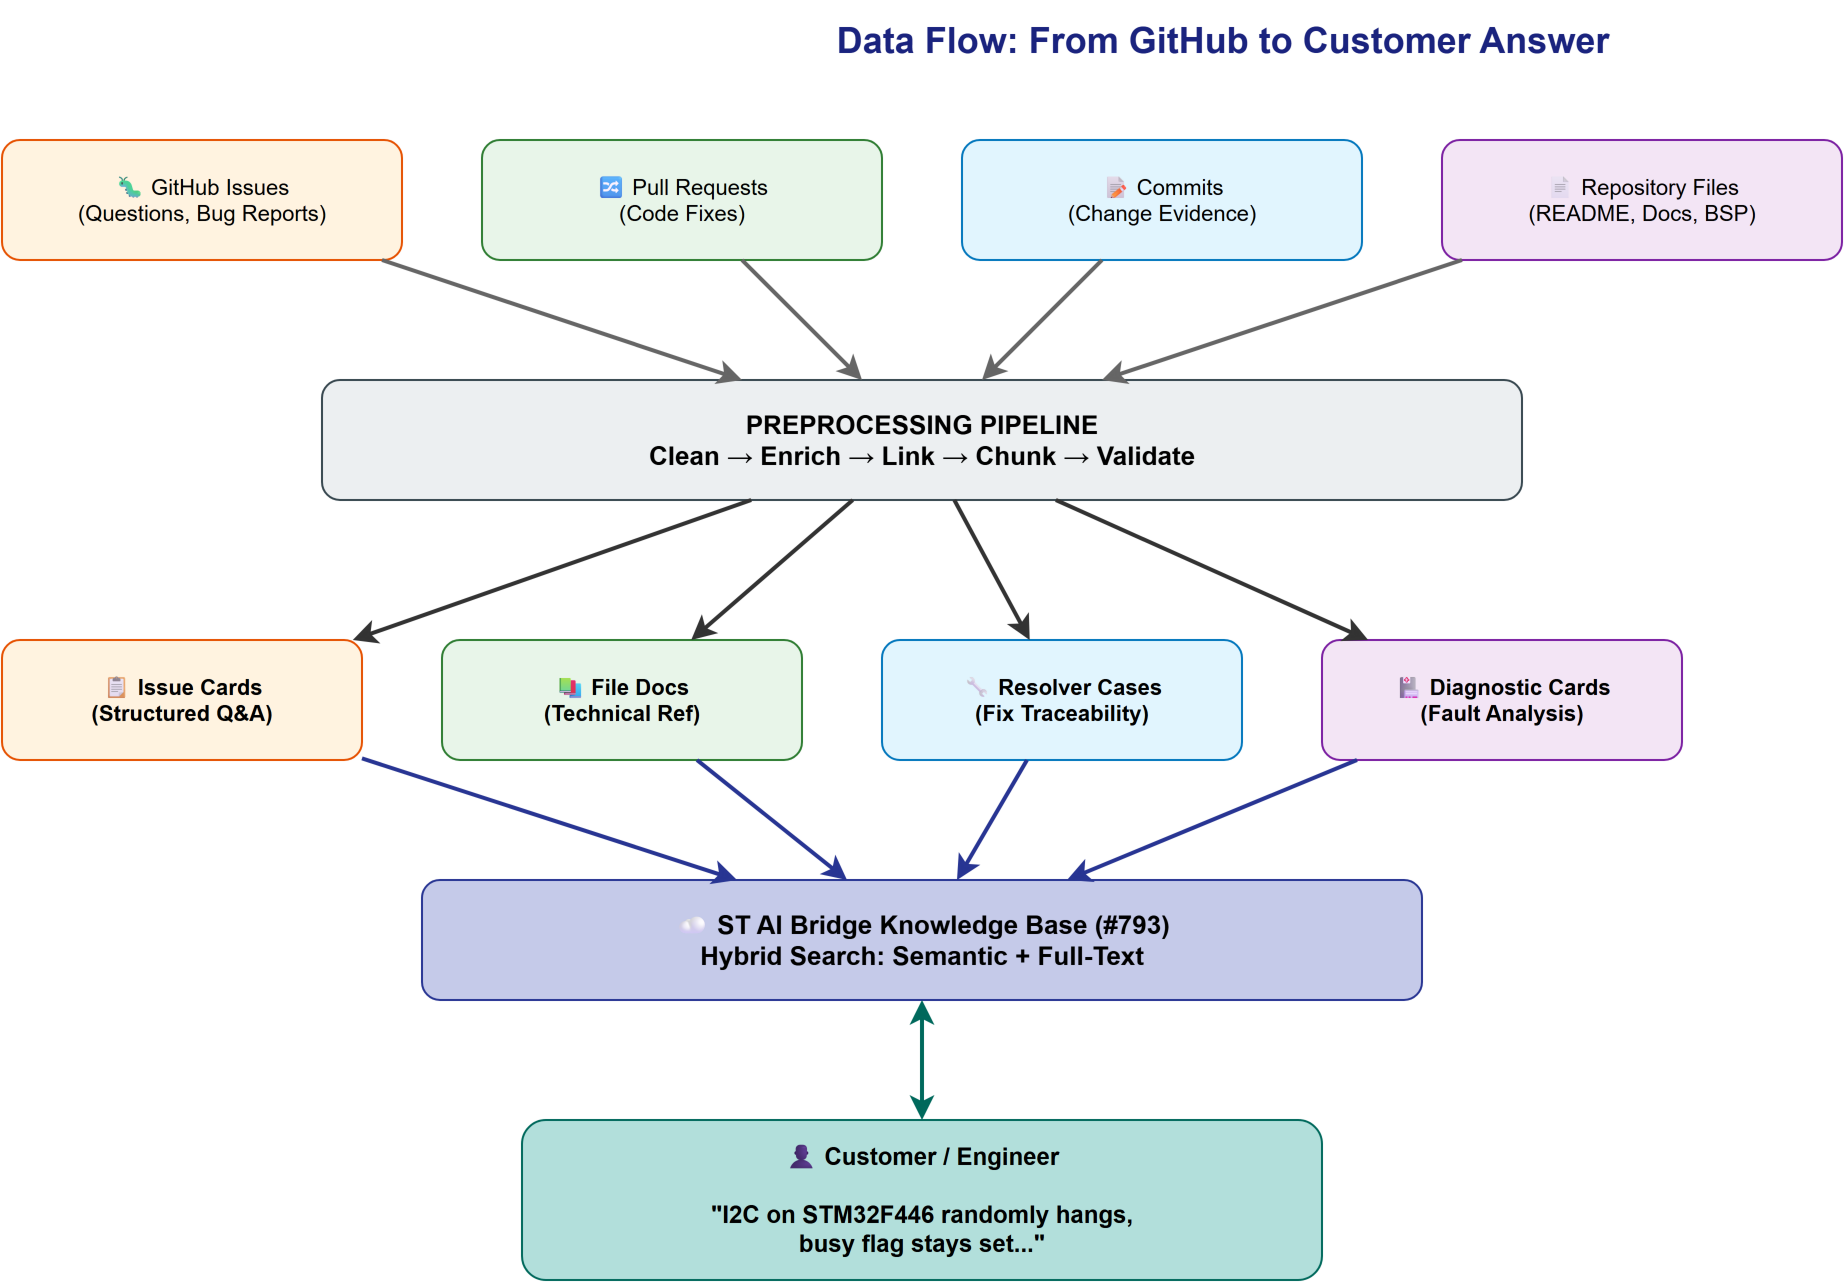
\includegraphics[width=\textwidth]{03_data_flow_source_to_answer.png}
  \caption{End-to-end data flow: from GitHub sources to chatbot answers}
  \label{fig:data-flow-overview}
\end{figure}

%% ============================================================
\chapter{Architecture}
%% ============================================================

\section{Pipeline Stages}

The pipeline consists of 7 sequential stages, each reading from the previous stage's output:

\begin{figure}[H]
  \centering
  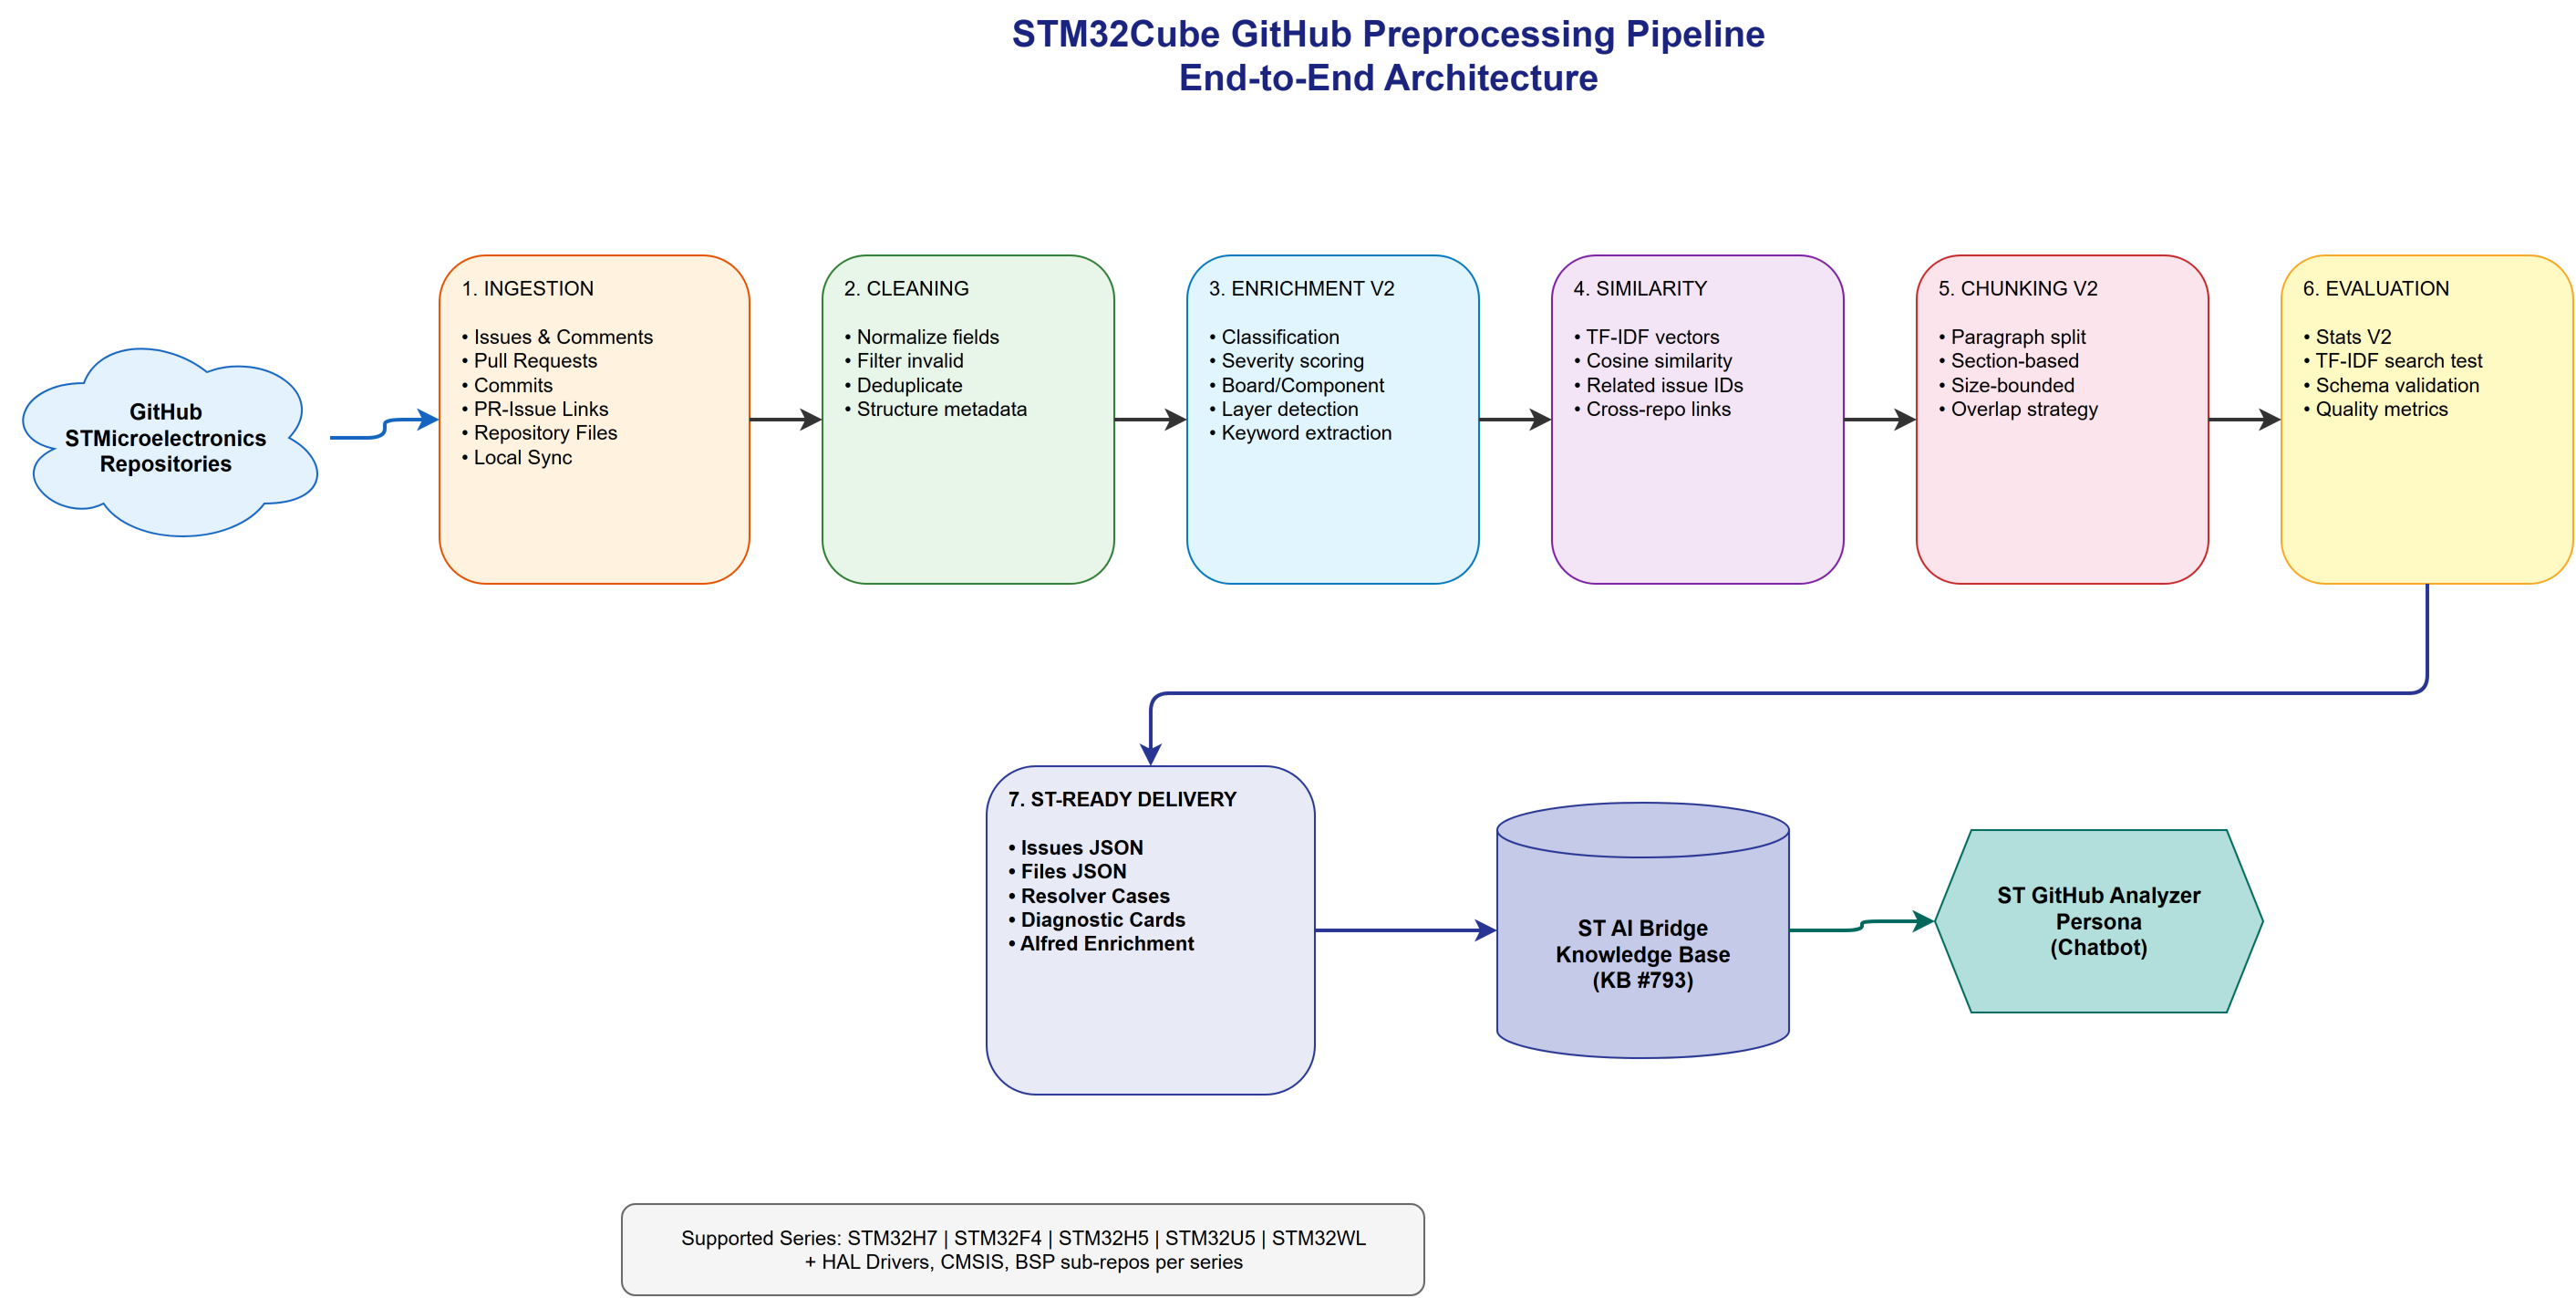
\includegraphics[width=\textwidth]{01_pipeline_overview.png}
  \caption{High-level pipeline architecture: 7 sequential stages}
  \label{fig:pipeline-overview}
\end{figure}

\begin{enumerate}
  \item \textbf{Ingestion} --- Fetch raw data from GitHub API and local clones
  \item \textbf{Cleaning} --- Normalize, deduplicate, structure metadata
  \item \textbf{Enrichment V2} --- Classify issues/files with heuristic NLP
  \item \textbf{Similarity} --- Compute TF-IDF cross-issue similarity
  \item \textbf{Chunking V2} --- Split documents for optimal retrieval
  \item \textbf{Evaluation} --- Stats, TF-IDF search tests, schema validation
  \item \textbf{Delivery} --- Export ST-ready JSON for KB upload
\end{enumerate}

\section{Repository Structure}

\begin{lstlisting}[language=bash]
PFE_Chatbot_STM32Cube/
|-- pipeline/                  # Core pipeline stages
|   |-- ingestion/             # GitHub API fetchers
|   |-- cleaning/              # Data normalization
|   |-- enrichment/            # NLP classification
|   |-- similarity/            # TF-IDF similarity
|   |-- chunking/              # Document splitting
|   |-- evaluation/            # Quality testing
|   |-- delivery/              # ST-ready export
|   +-- run_full_workflow.py   # Orchestrator
|-- pipeline_Automation/       # Upload & batch scripts
|-- shared/
|   |-- config/                # Per-series config files
|   |-- schemas/               # JSON Schema definitions
|   +-- utils/                 # Path helpers, utilities
|-- datasets/
|   |-- 01_raw/                # Raw ingested data
|   +-- 07_delivery/st_ready/  # Final delivery outputs
|       +-- by_series/         # Organized per MCU series
|-- GitHub_repos/              # Local cloned repositories
|-- docs/                      # Documentation & diagrams
+-- data/                      # Historical/intermediate
\end{lstlisting}

\begin{figure}[H]
  \centering
  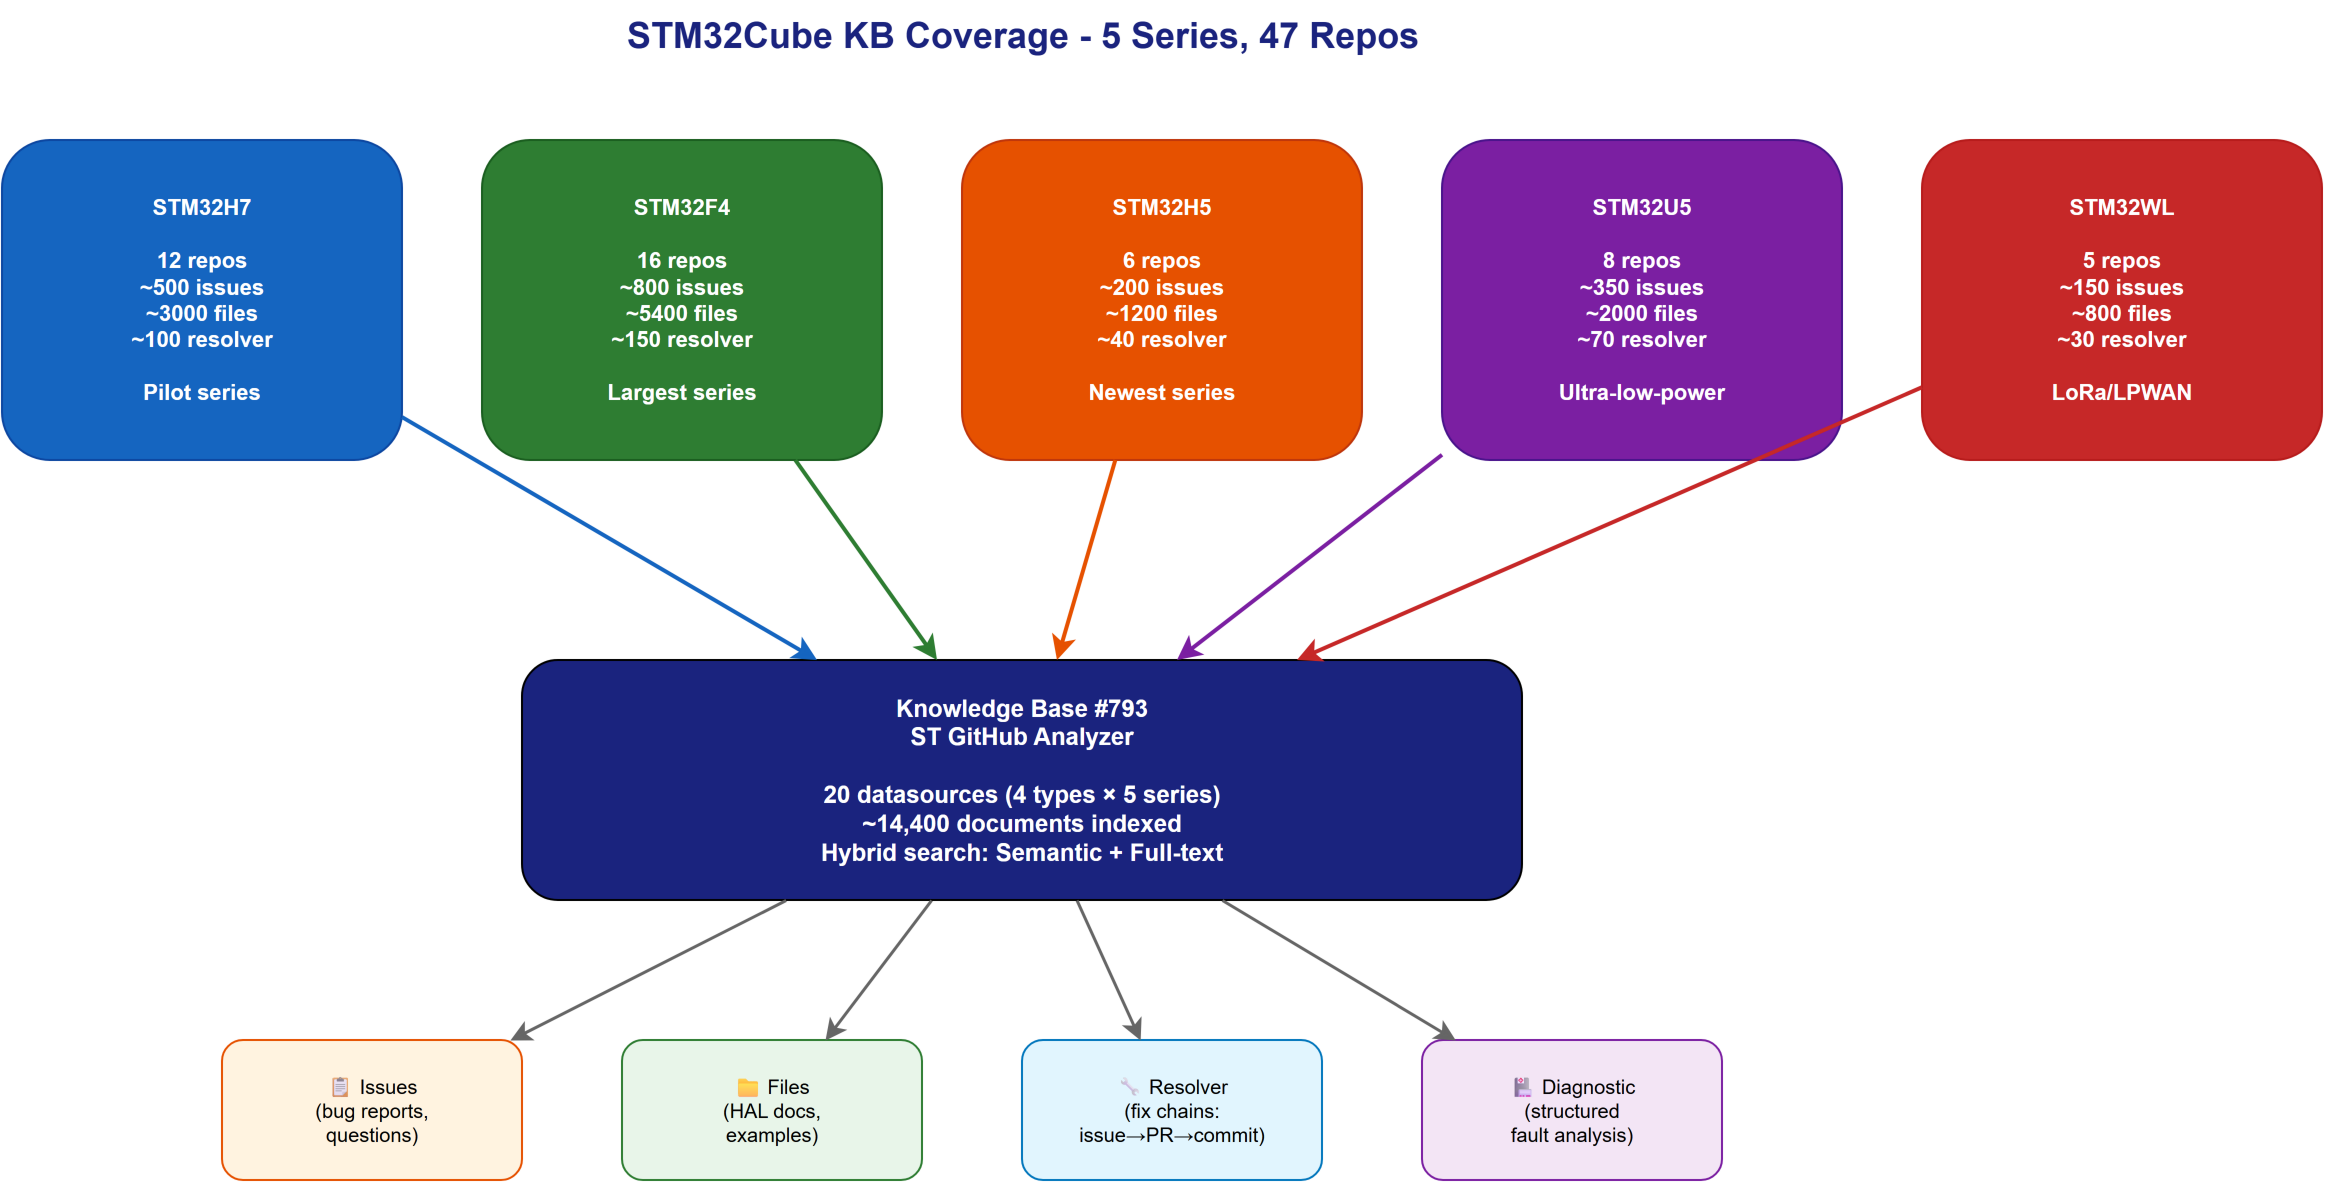
\includegraphics[width=0.85\textwidth]{04_series_coverage_scale.png}
  \caption{Multi-series coverage: 5 MCU families, 40+ repositories}
  \label{fig:series-coverage}
\end{figure}

\section{Configuration System}

Each MCU series has a dedicated configuration file:

\begin{itemize}
  \item \texttt{shared/config/config.json} --- Default (H7, 12 repos)
  \item \texttt{shared/config/config\_f4.json} --- STM32F4 (16 repos)
  \item \texttt{shared/config/config\_h5.json} --- STM32H5 (6 repos)
  \item \texttt{shared/config/config\_u5.json} --- STM32U5 (8 repos)
  \item \texttt{shared/config/config\_wl.json} --- STM32WL (5 repos)
\end{itemize}

%% ============================================================
\chapter{Pipeline Stage Details}
%% ============================================================

\section{Stage 1: Ingestion}

\begin{figure}[H]
  \centering
  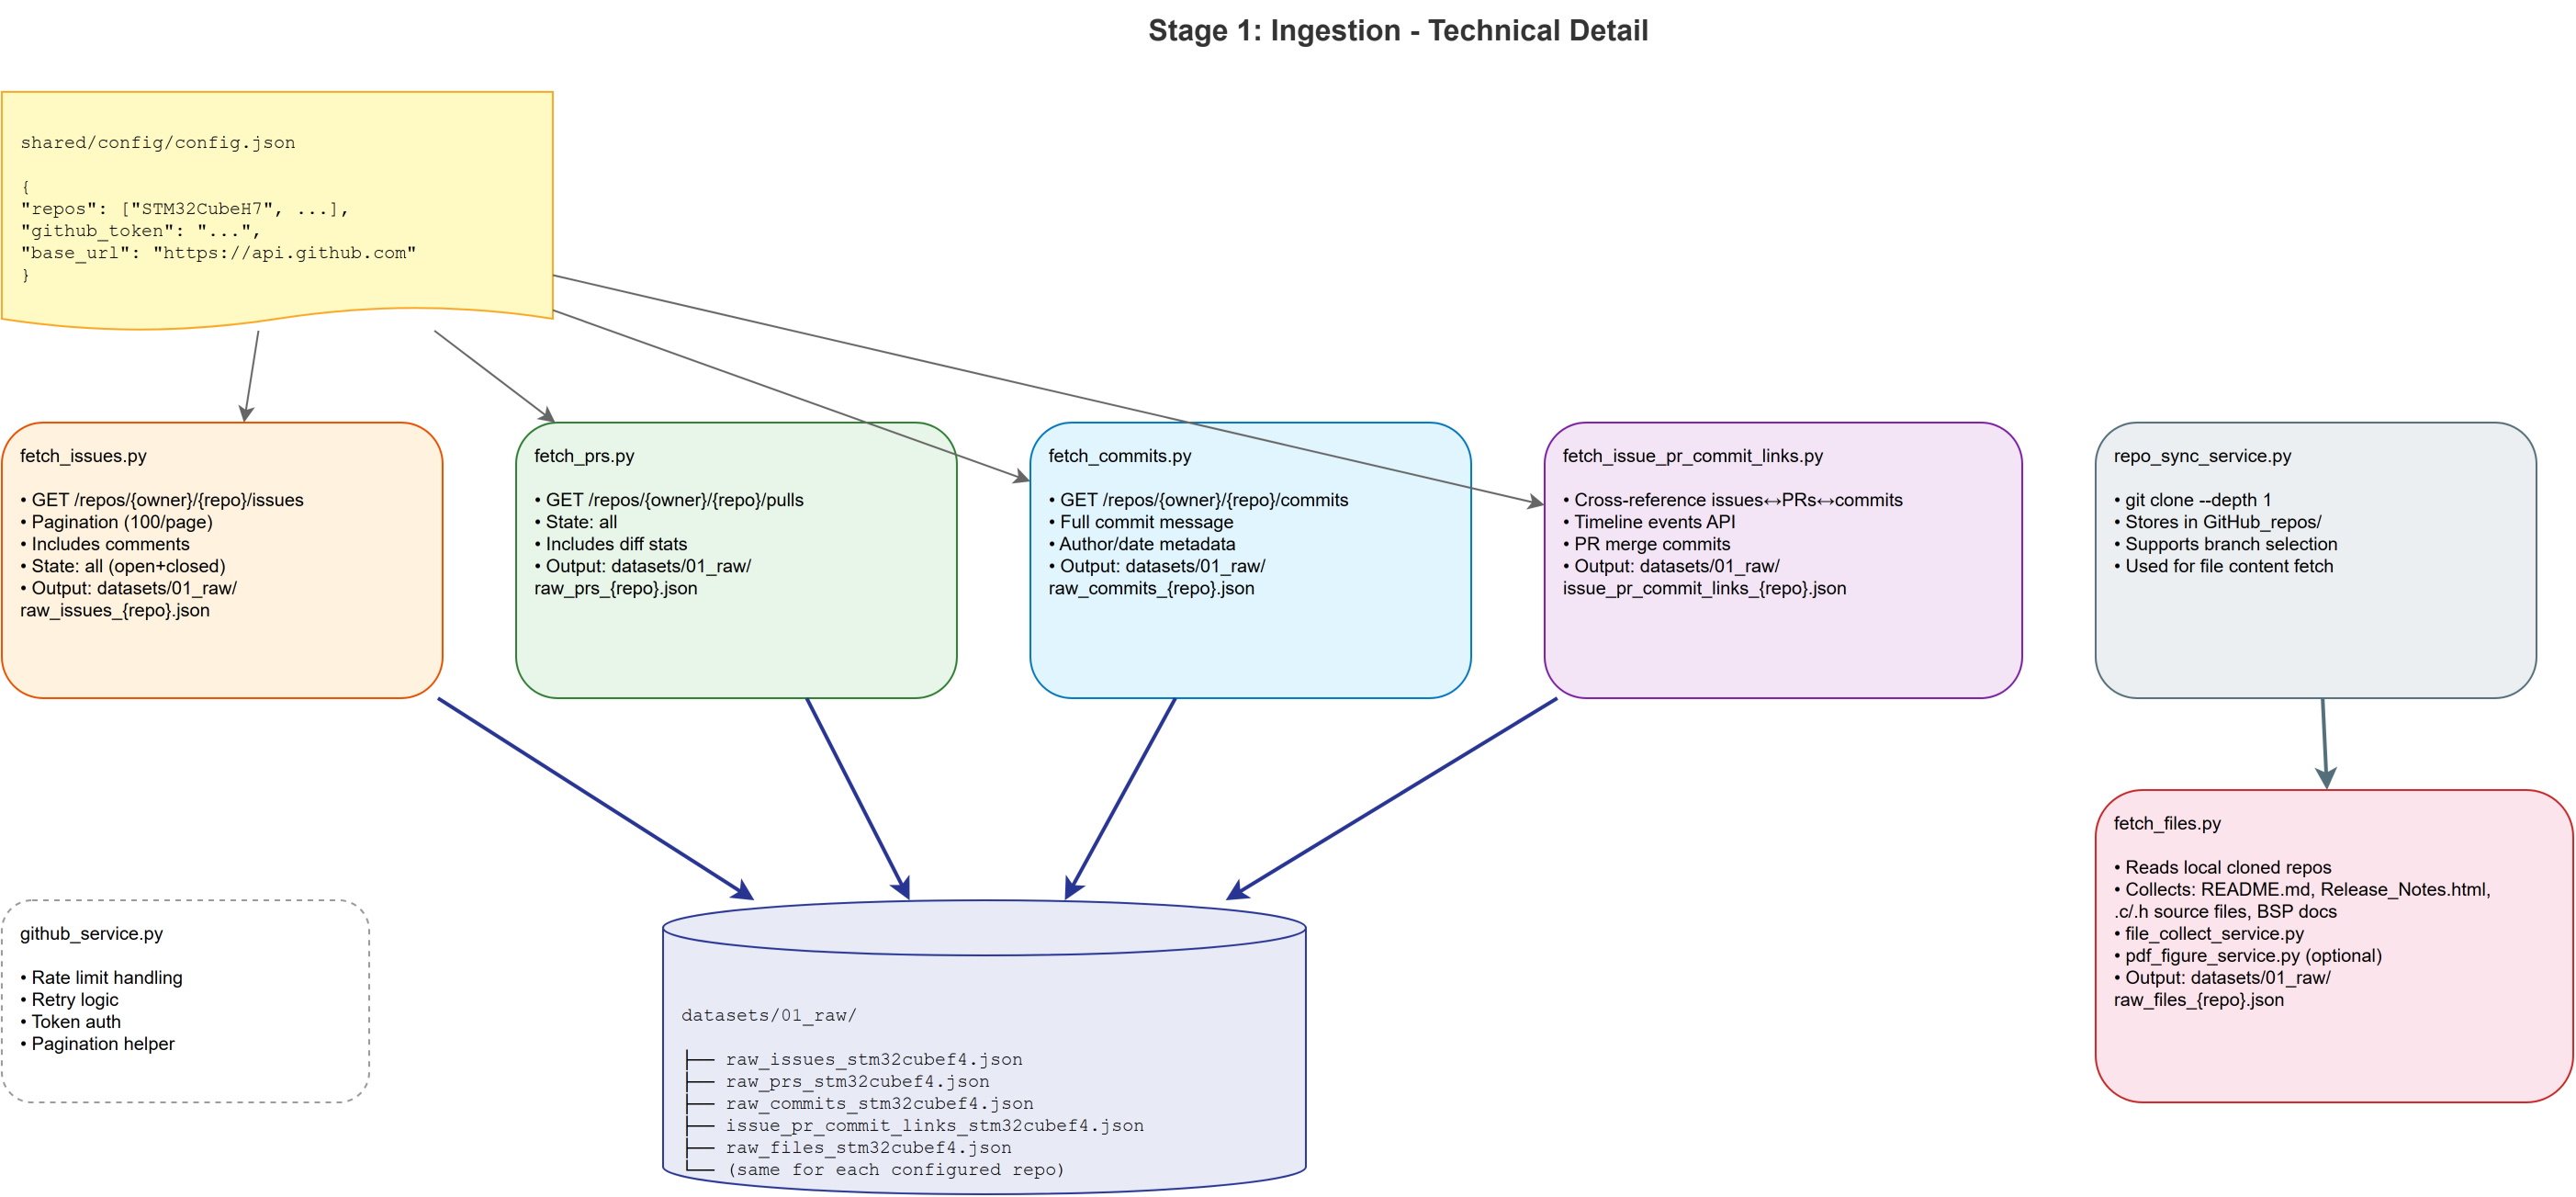
\includegraphics[width=\textwidth]{01_ingestion_detail.png}
  \caption{Ingestion stage: scripts, API calls, and output artifacts}
  \label{fig:ingestion-detail}
\end{figure}

\subsection{Scripts}

\begin{longtable}{p{5cm}p{9cm}}
\toprule
\textbf{Script} & \textbf{Function} \\
\midrule
\texttt{fetch\_issues.py} & Fetch all issues (open+closed) with comments \\
\texttt{fetch\_prs.py} & Fetch pull requests with diff stats \\
\texttt{fetch\_commits.py} & Fetch commits with messages \\
\texttt{fetch\_issue\_pr\_commit\_links.py} & Cross-reference issues$\leftrightarrow$PRs$\leftrightarrow$commits \\
\texttt{repo\_sync\_service.py} & Git clone/pull repositories locally \\
\texttt{fetch\_files.py} & Extract file content from local clones \\
\texttt{github\_service.py} & Shared: auth, rate-limiting, pagination \\
\bottomrule
\end{longtable}

\subsection{Output}
All raw data is stored in \texttt{datasets/01\_raw/} as JSON files named \texttt{raw\_\{type\}\_\{repo\}.json}.

\section{Stage 2: Cleaning}

\begin{itemize}
  \item \texttt{clean\_issues.py} --- Normalize issue fields, filter spam, deduplicate
  \item \texttt{clean\_files.py} --- Normalize file paths, filter binary/irrelevant files
\end{itemize}

Output: \texttt{data/clean\_issues\_\{repo\}.json}, \texttt{data/clean\_files\_\{repo\}.json}

\section{Stage 3: Enrichment V2}

\begin{figure}[H]
  \centering
  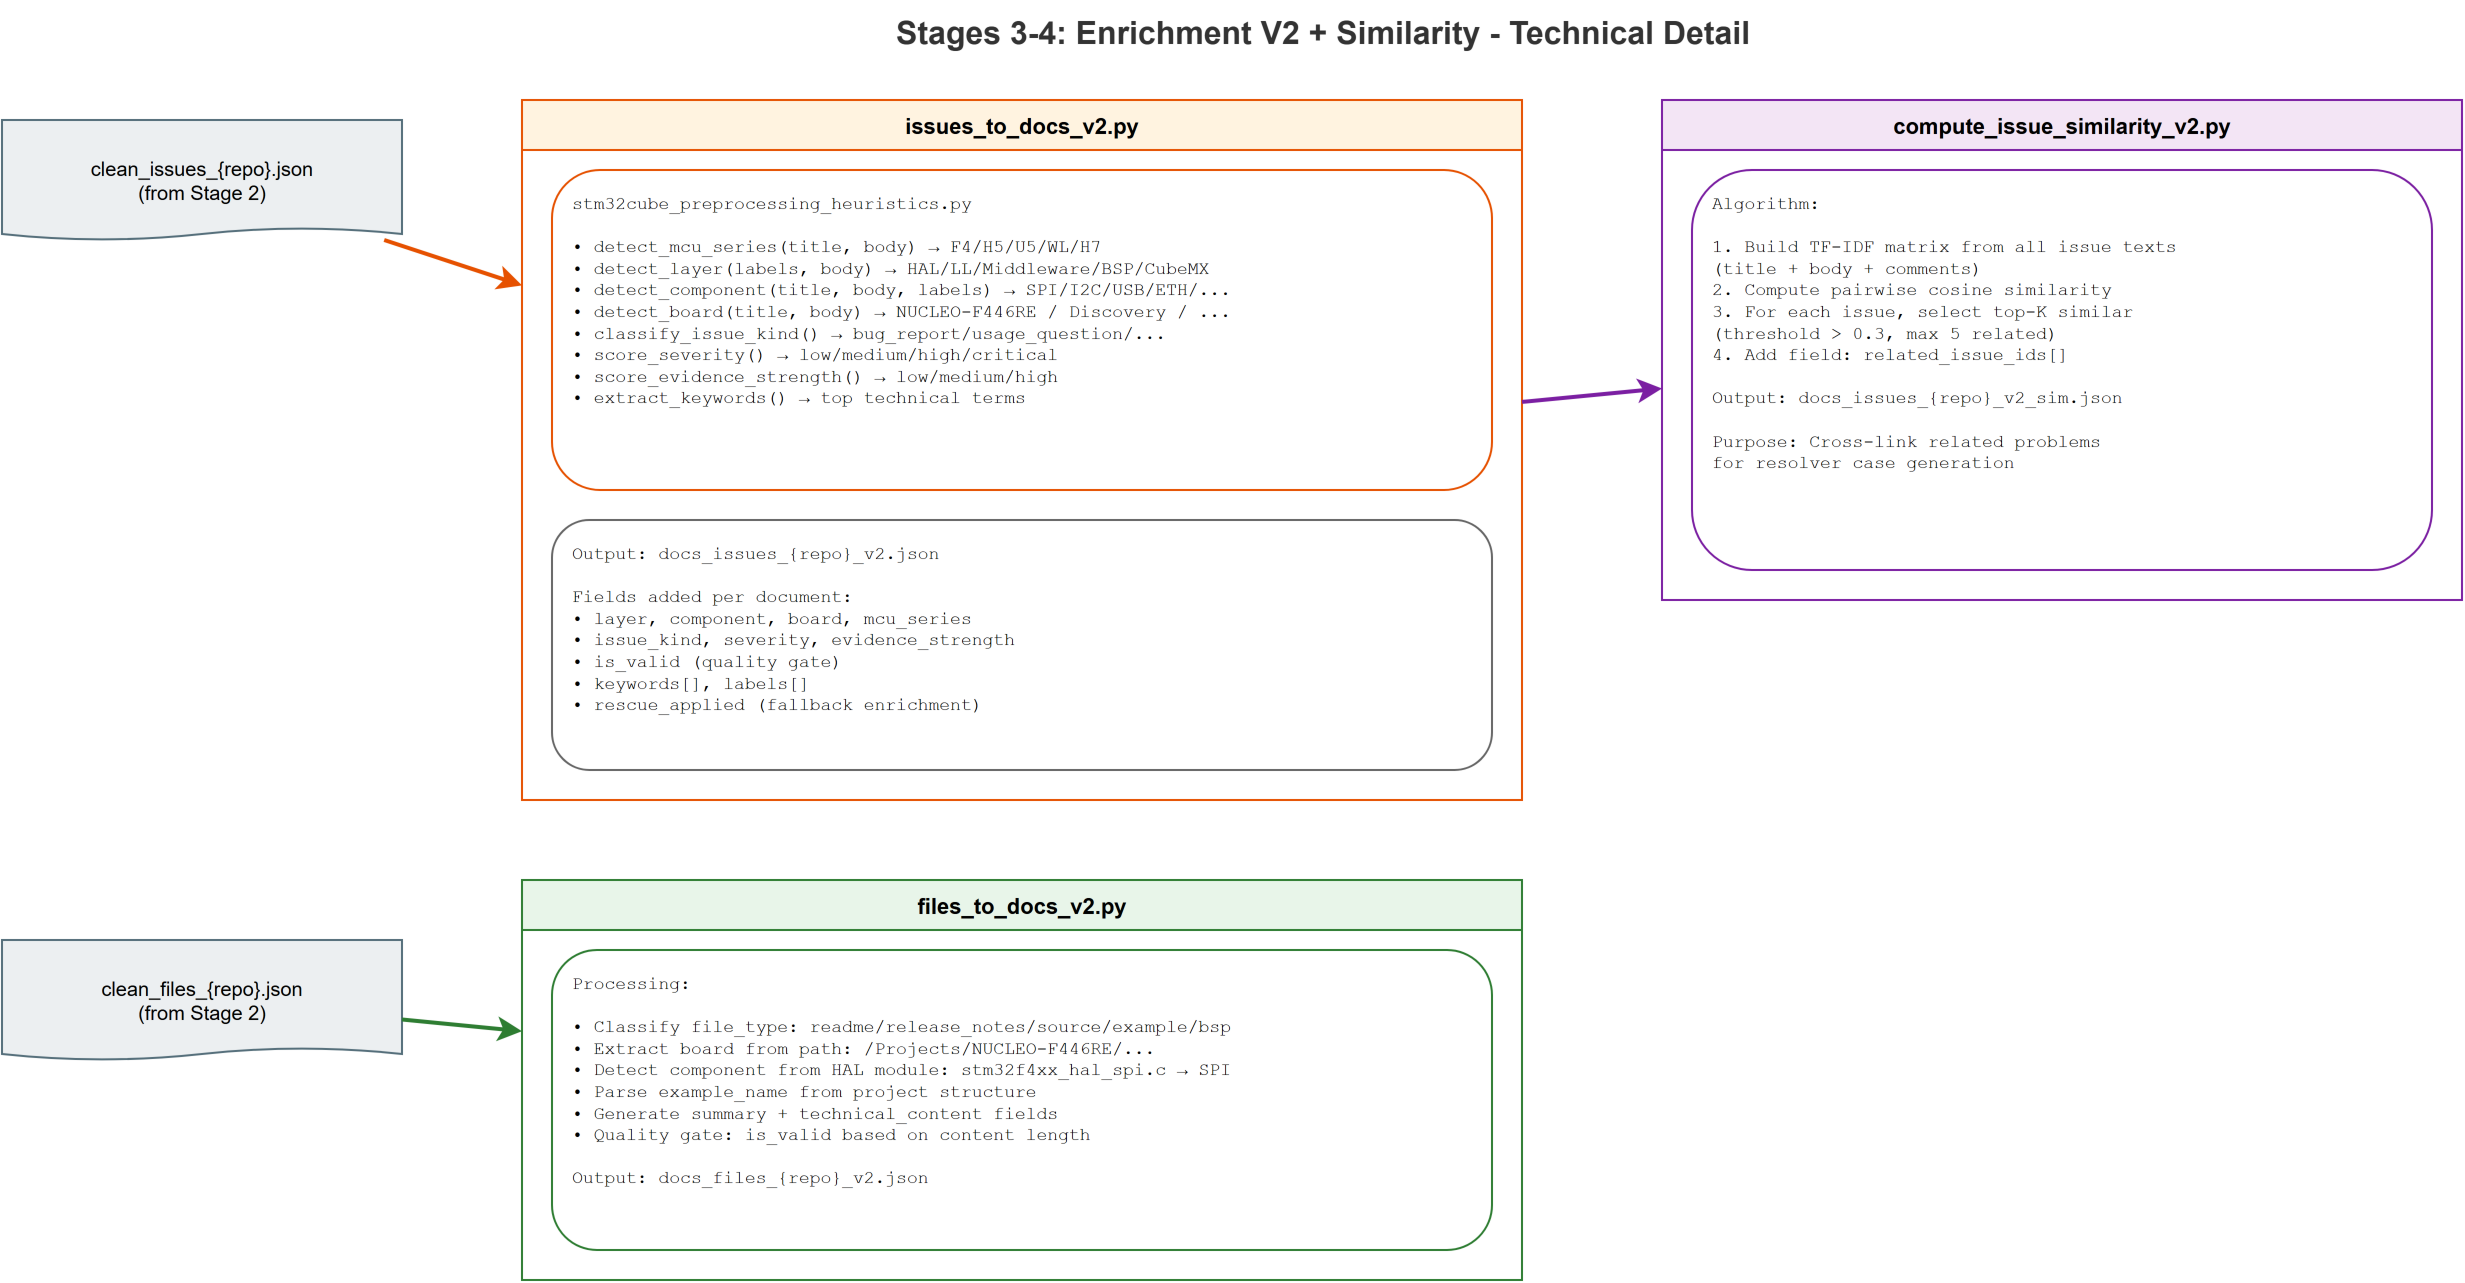
\includegraphics[width=\textwidth]{02_enrichment_similarity_detail.png}
  \caption{Enrichment \& similarity stage: heuristic NLP classification and TF-IDF cross-linking}
  \label{fig:enrichment-detail}
\end{figure}

\subsection{Issues Enrichment (\texttt{issues\_to\_docs\_v2.py})}

Uses \texttt{stm32cube\_preprocessing\_heuristics.py} to classify each issue:

\begin{longtable}{p{4cm}p{4cm}p{5cm}}
\toprule
\textbf{Field} & \textbf{Type} & \textbf{Values} \\
\midrule
\texttt{mcu\_series} & string & F4, H5, H7, U5, WL \\
\texttt{layer} & string & HAL, LL, Middleware, BSP, CubeMX, Other \\
\texttt{component} & string & SPI, I2C, USB, ETH, DMA, ADC, ... \\
\texttt{board} & string & NUCLEO-F446RE, Discovery, ... \\
\texttt{issue\_kind} & string & bug\_report, usage\_question, config\_help, other \\
\texttt{severity} & string & low, medium, high, critical \\
\texttt{evidence\_strength} & string & low, medium, high \\
\texttt{is\_valid} & boolean & Quality gate for delivery \\
\texttt{keywords} & string[] & Top technical terms \\
\texttt{rescue\_applied} & boolean & Fallback enrichment used \\
\bottomrule
\end{longtable}

\subsection{Files Enrichment (\texttt{files\_to\_docs\_v2.py})}

Classifies repository files by type, board, component, and extracts structured content.

\section{Stage 4: Similarity}

\texttt{compute\_issue\_similarity\_v2.py}:
\begin{enumerate}
  \item Builds TF-IDF matrix from issue text corpus
  \item Computes pairwise cosine similarity
  \item Attaches \texttt{related\_issue\_ids[]} (top-5, threshold $> 0.3$)
\end{enumerate}

Output: \texttt{docs\_issues\_\{repo\}\_v2\_sim.json}

\section{Stage 5: Chunking V2}

\begin{itemize}
  \item \texttt{docs\_to\_chunks\_issues\_v2.py} --- Paragraph-based chunking with overlap
  \item \texttt{docs\_to\_chunks\_files\_v2.py} --- Section-based chunking for file docs
\end{itemize}

Strategy: bounded chunks (max 512 tokens) with 50-token overlap for context continuity.

\section{Stage 6: Evaluation}

\begin{longtable}{p{5cm}p{8cm}}
\toprule
\textbf{Script} & \textbf{Purpose} \\
\midrule
\texttt{test\_stats\_issues\_v2.py} & Distribution analysis: severity, layer, component \\
\texttt{test\_stats\_files\_v2.py} & File type distribution, board coverage \\
\texttt{test\_tfidf\_search\_issues\_v2.py} & TF-IDF retrieval precision testing \\
\texttt{test\_tfidf\_search\_files\_v2.py} & File retrieval precision testing \\
\texttt{validate\_schemas.py} & JSON Schema validation gate \\
\bottomrule
\end{longtable}

\section{Stage 7: Delivery}

\begin{figure}[H]
  \centering
  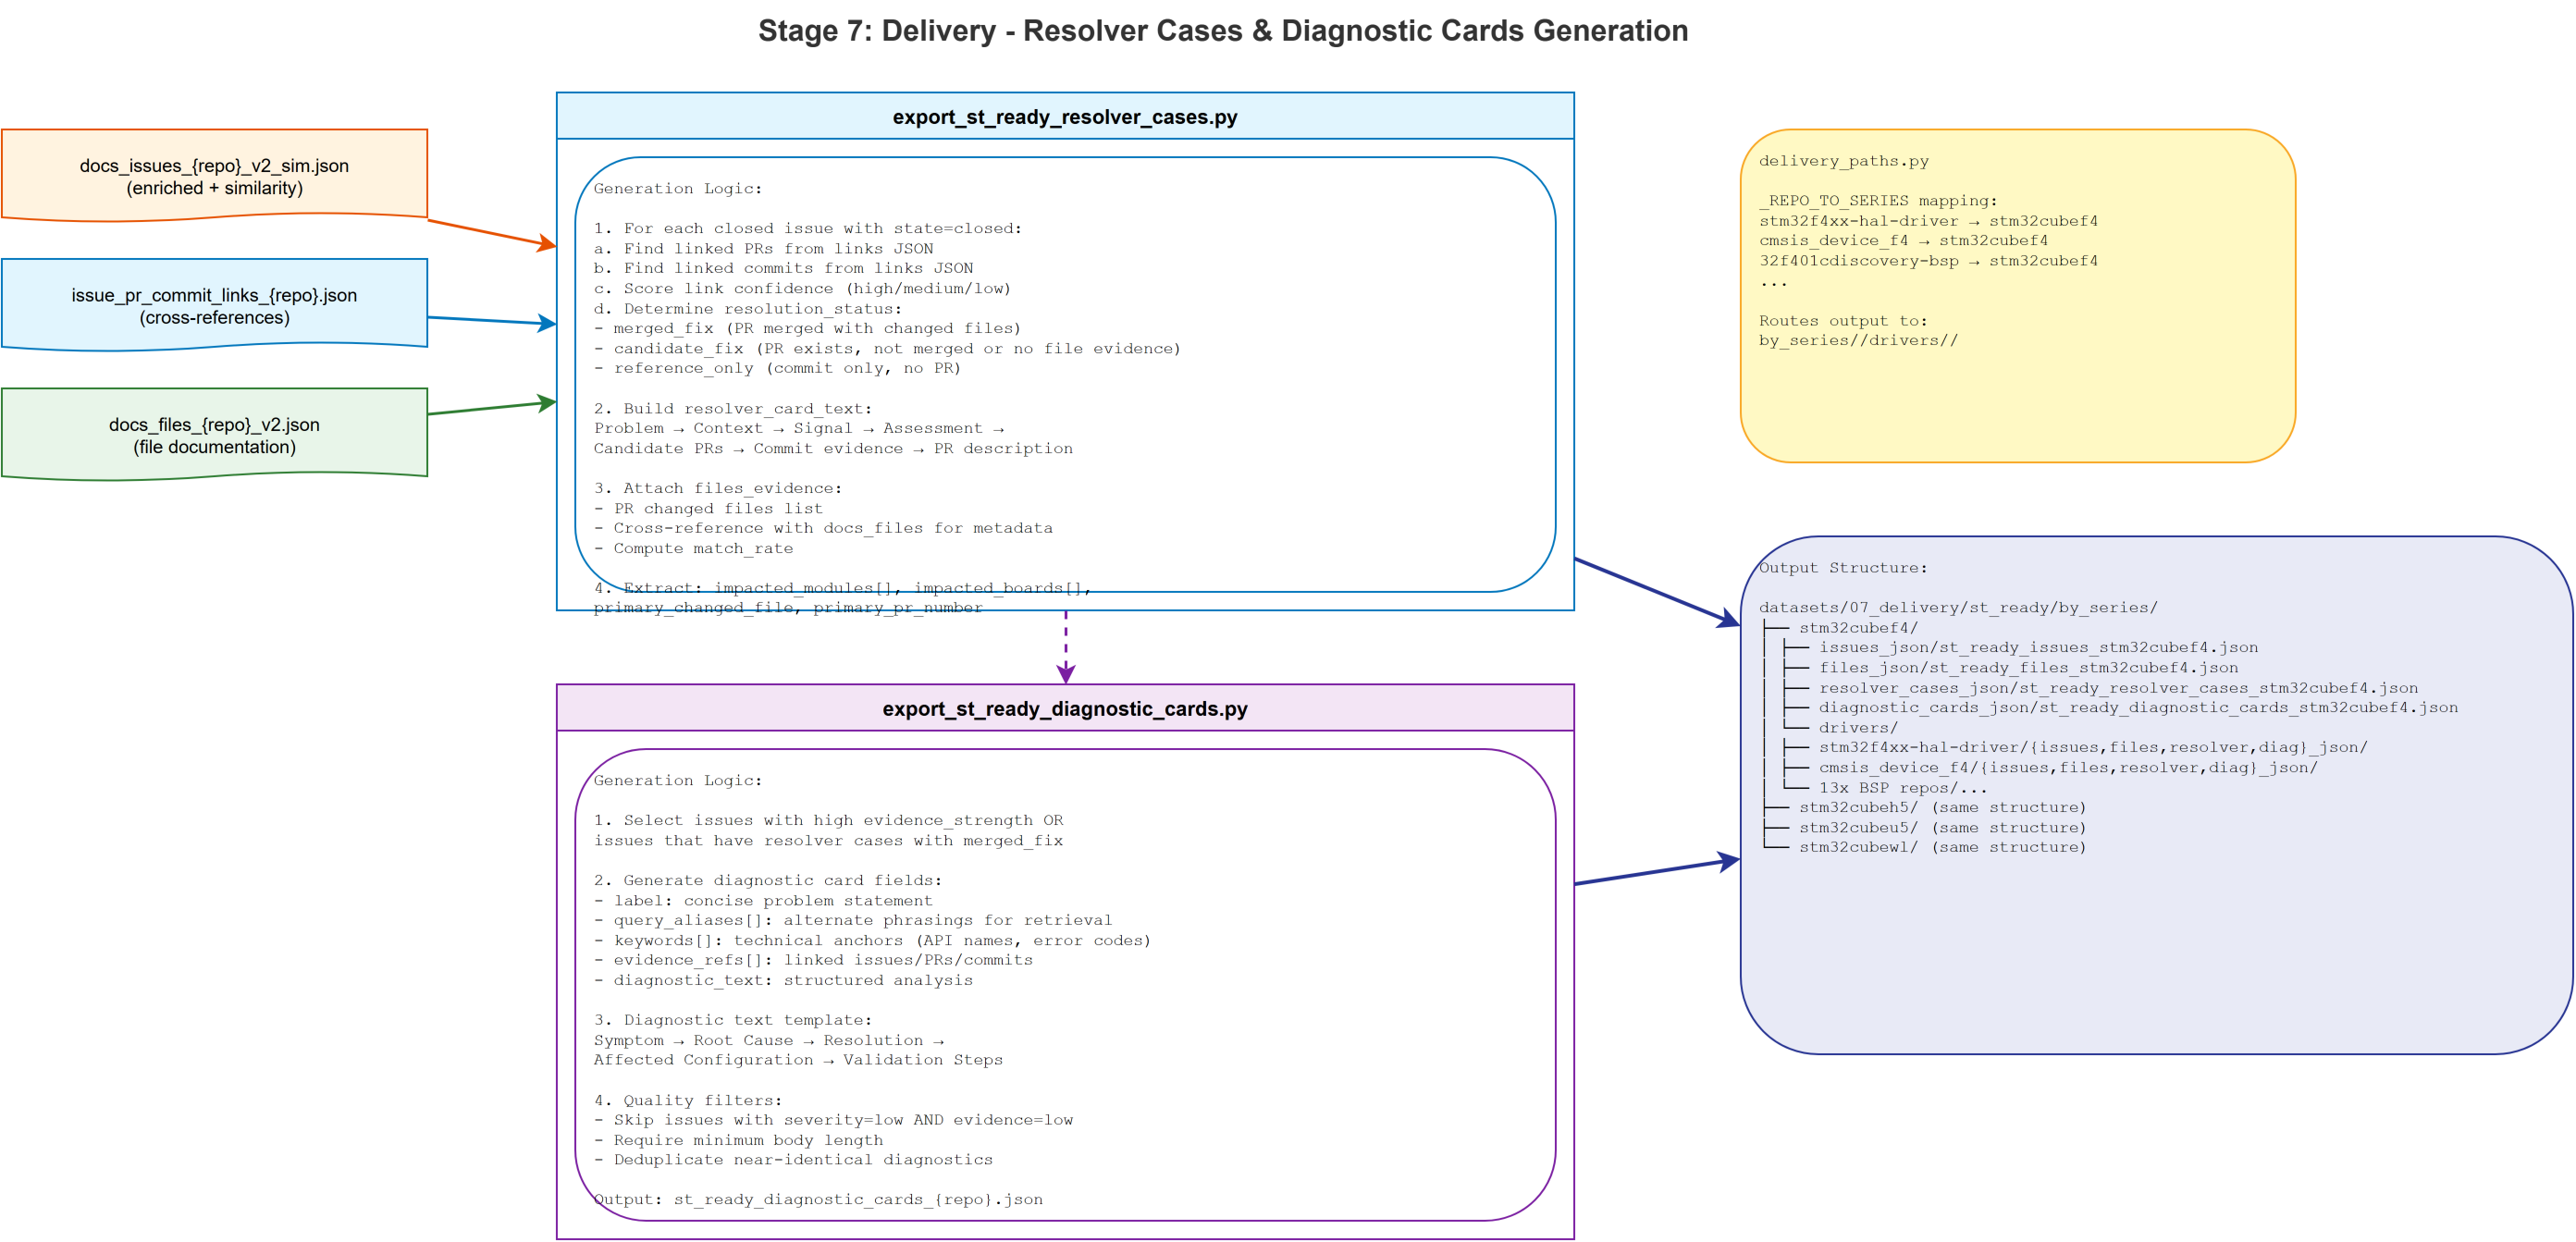
\includegraphics[width=\textwidth]{03_delivery_resolver_diagnostic.png}
  \caption{Delivery stage: resolver cases and diagnostic card generation}
  \label{fig:delivery-resolver}
\end{figure}

\begin{figure}[H]
  \centering
  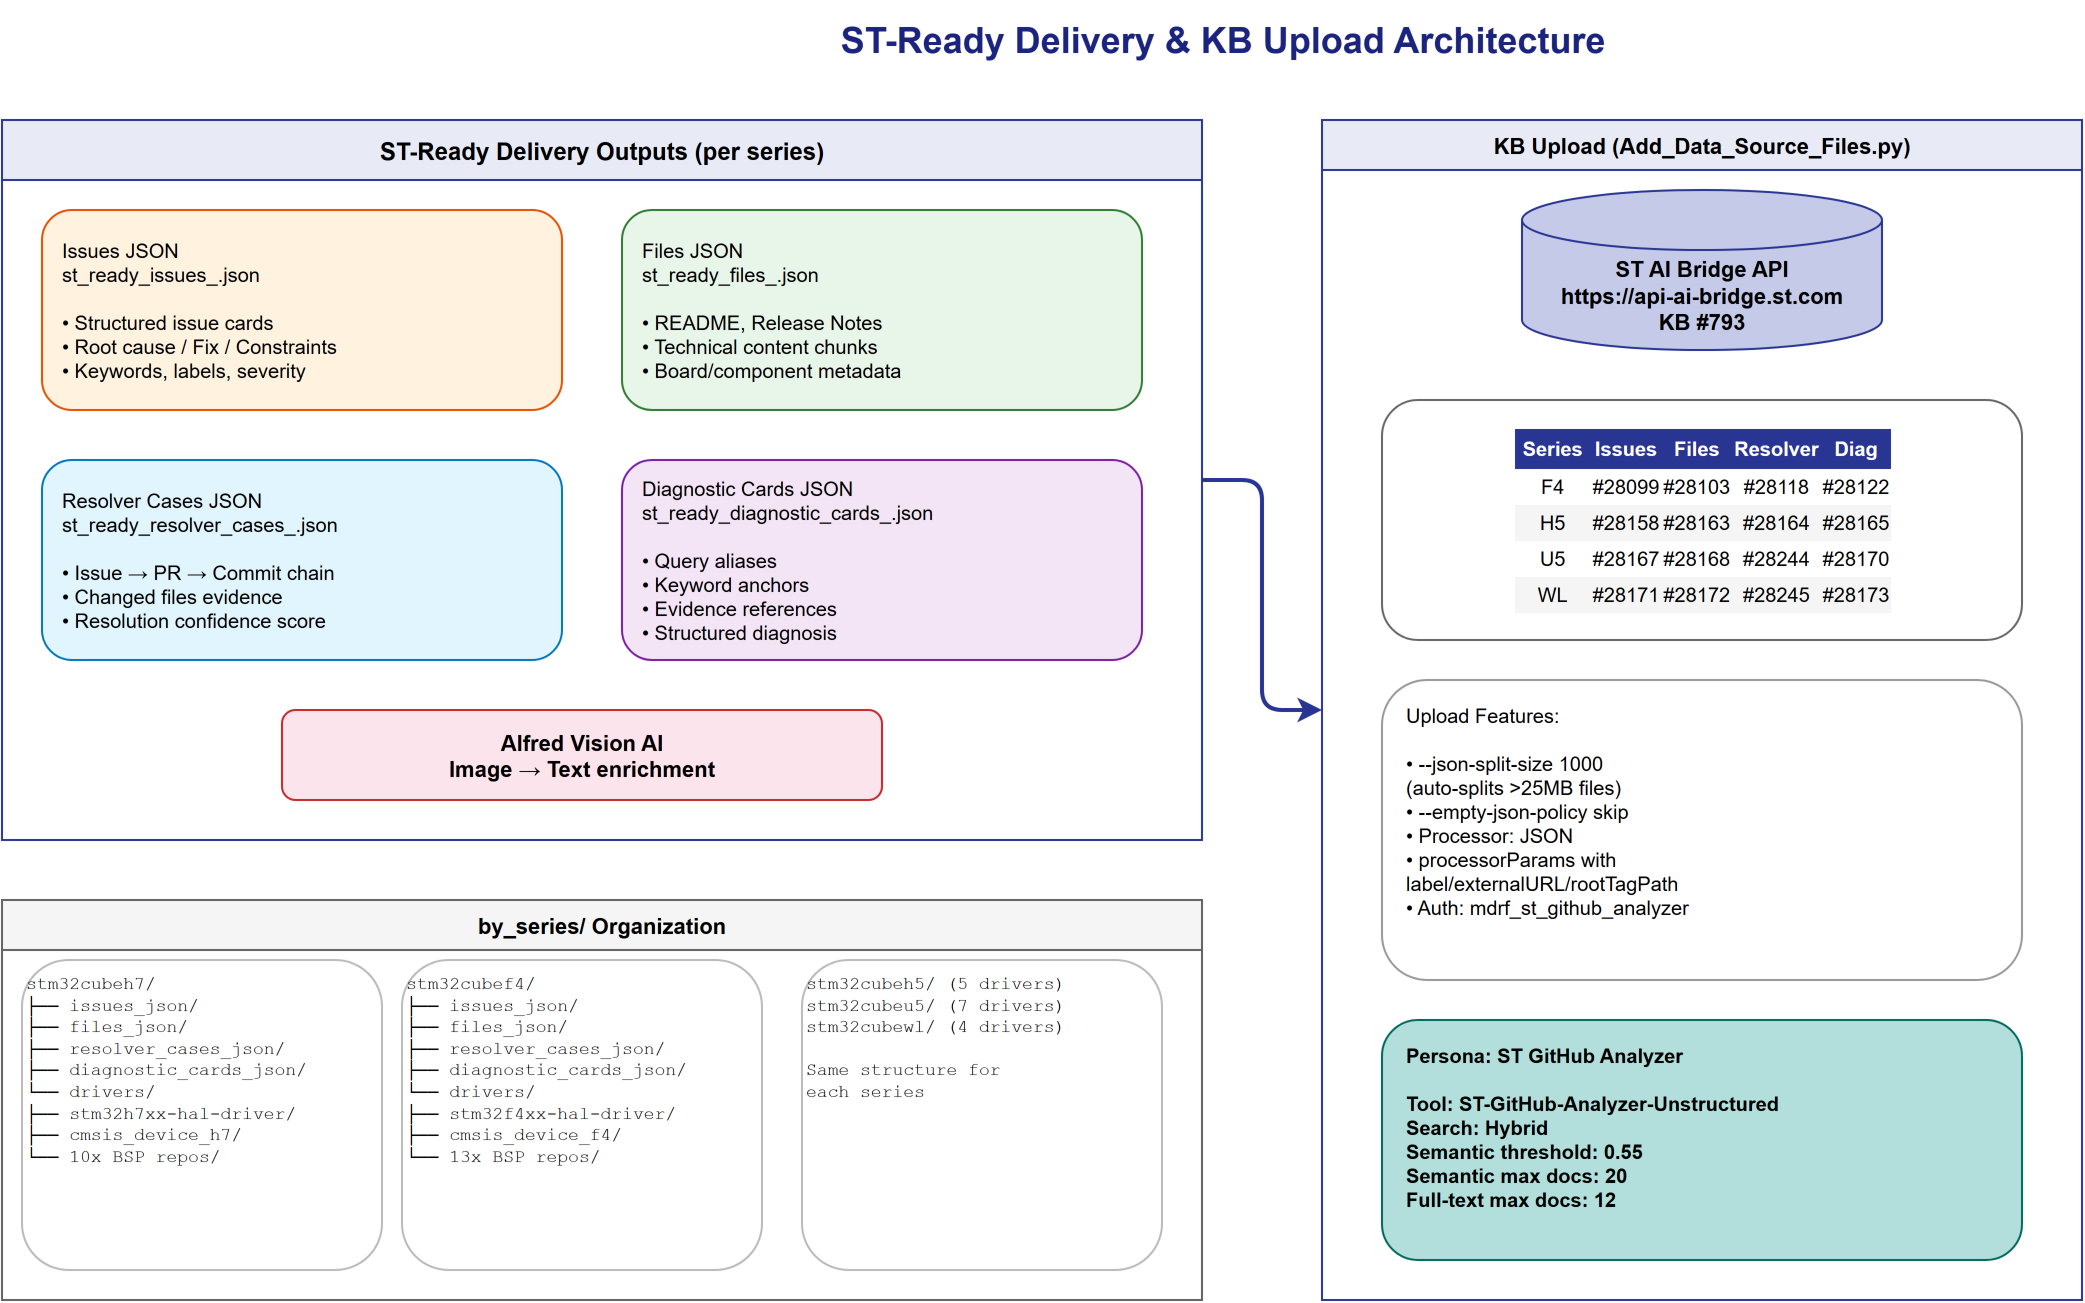
\includegraphics[width=\textwidth]{02_delivery_kb_upload.png}
  \caption{Delivery artifacts and KB upload workflow}
  \label{fig:delivery-kb-upload}
\end{figure}

\subsection{Export Scripts}

\begin{itemize}
  \item \texttt{export\_st\_ready\_issues.py} --- Structured issue cards
  \item \texttt{export\_st\_ready\_files.py} --- Technical file documentation
  \item \texttt{export\_st\_ready\_resolver\_cases.py} --- Issue→PR→Commit fix chains
  \item \texttt{export\_st\_ready\_diagnostic\_cards.py} --- Structured fault analysis
\end{itemize}

\subsection{Delivery Path Routing}

\texttt{delivery\_paths.py} contains a \texttt{\_REPO\_TO\_SERIES} mapping that routes sub-repo outputs to the correct parent series folder:

\begin{verbatim}
by_series/stm32cubef4/drivers/stm32f4xx-hal-driver/issues_json/
by_series/stm32cubef4/drivers/cmsis_device_f4/files_json/
\end{verbatim}

%% ============================================================
\chapter{KB Upload \& Deployment}
%% ============================================================

\section{ST AI Bridge API}

\begin{figure}[H]
  \centering
  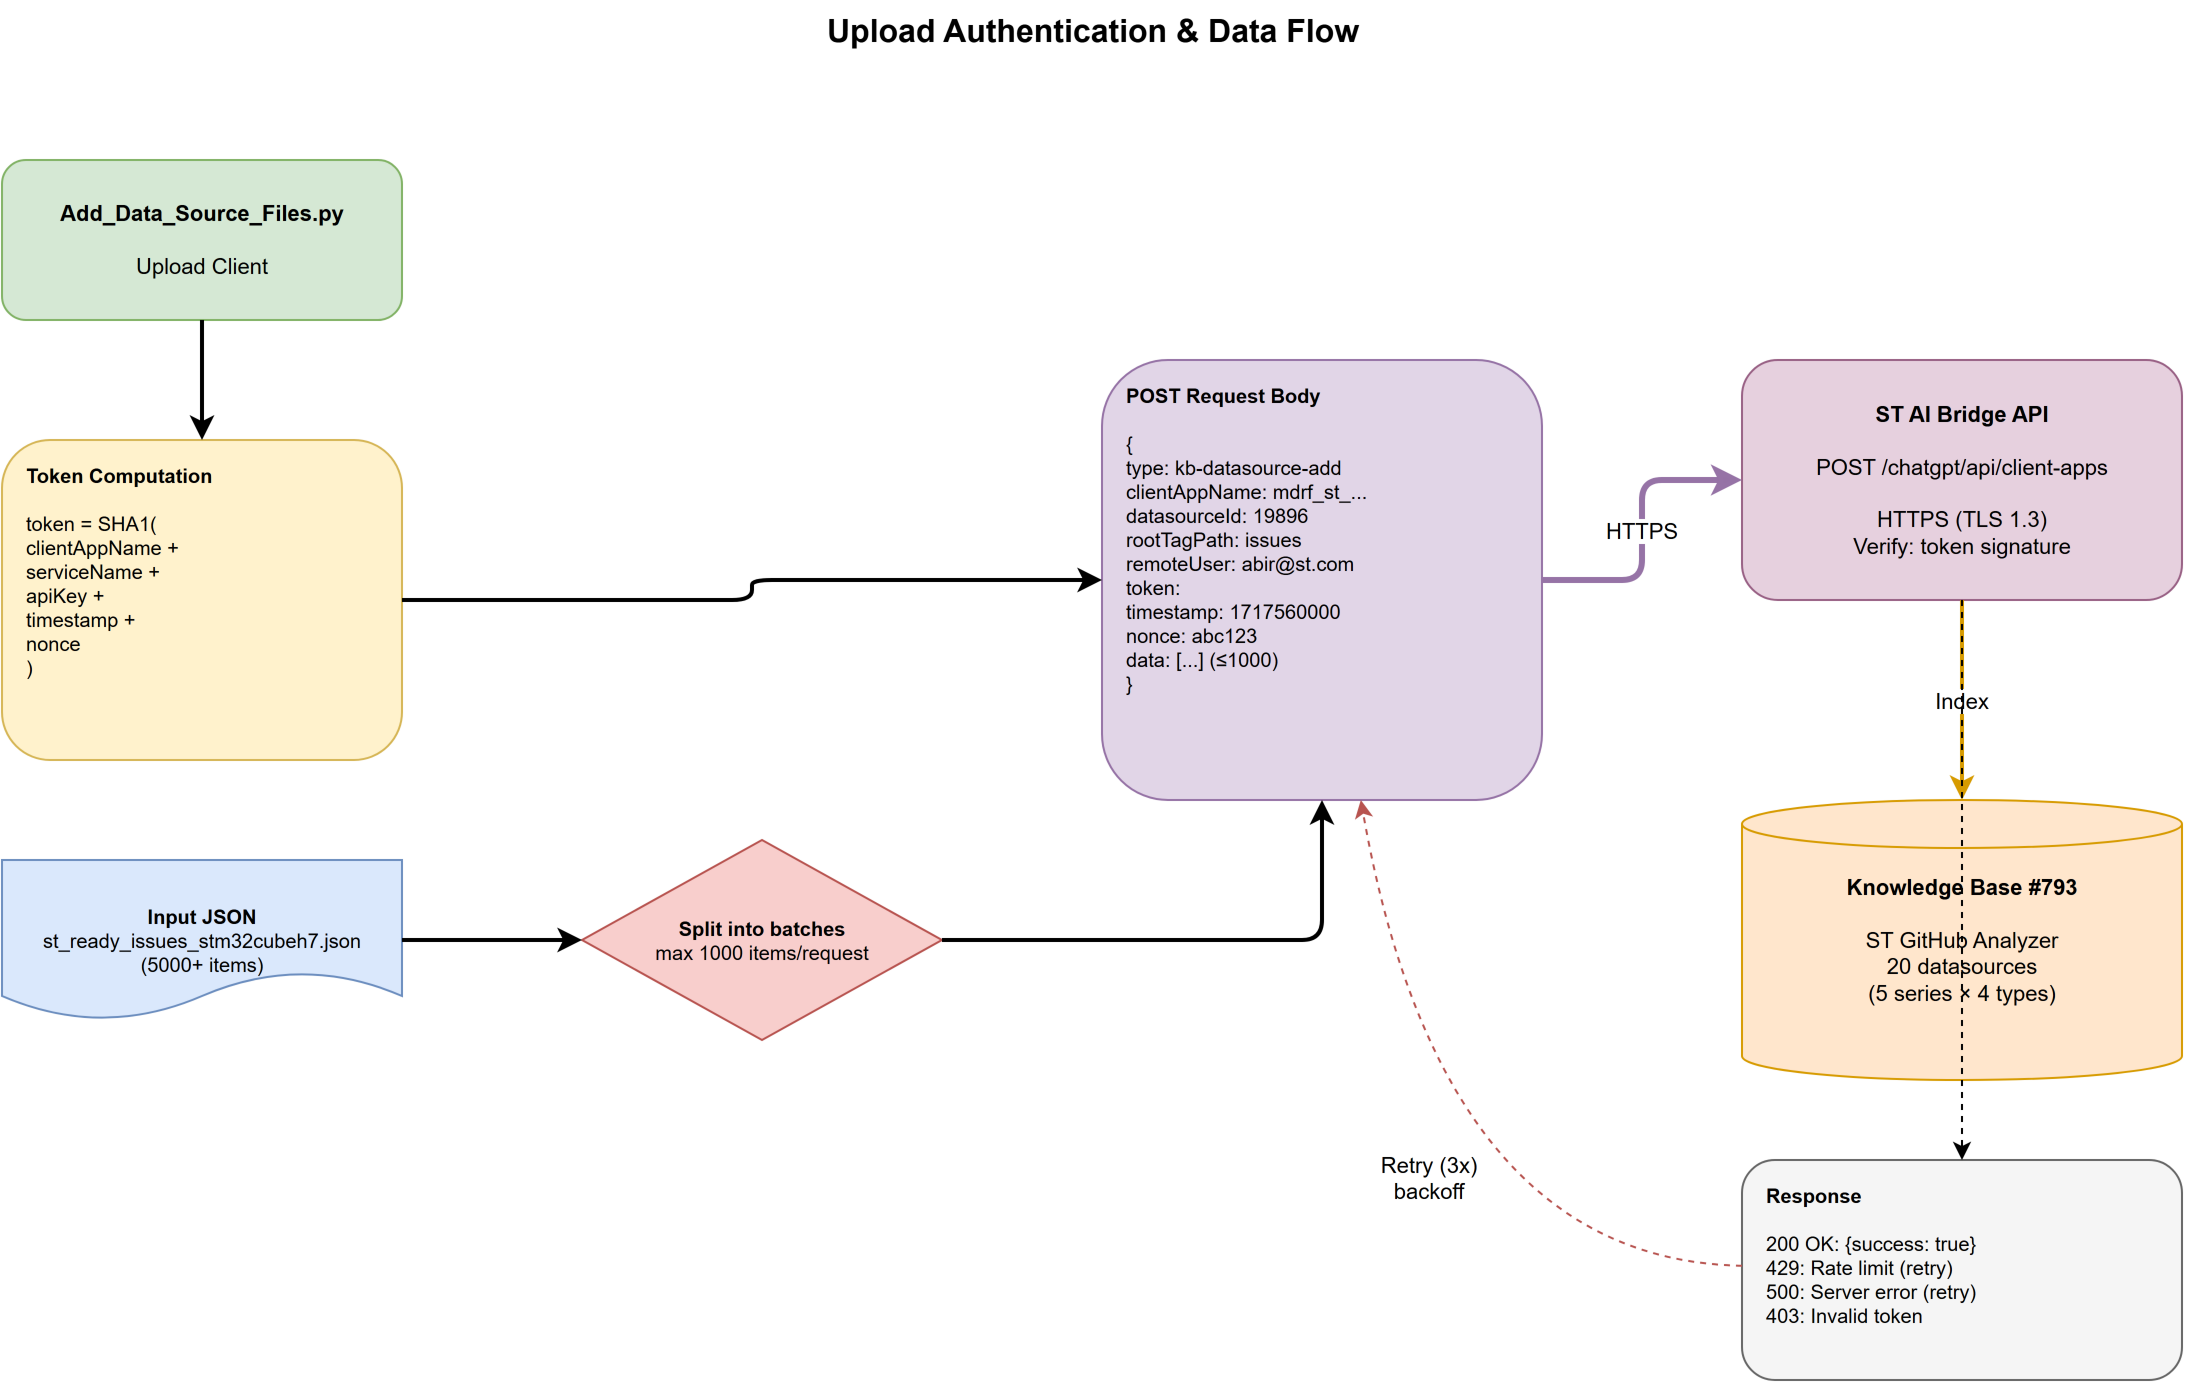
\includegraphics[width=0.9\textwidth]{07_upload_auth_flow.png}
  \caption{Upload authentication flow: API key, client app, and datasource creation}
  \label{fig:upload-auth-flow}
\end{figure}

\begin{itemize}
  \item \textbf{Endpoint}: \texttt{https://api-ai-bridge.st.com/chatgpt/api/client-apps}
  \item \textbf{KB ID}: 793 (ST GitHub Analyzer)
  \item \textbf{Auth}: clientAppName=\texttt{mdrf\_st\_github\_analyzer}
  \item \textbf{Upload tool}: \texttt{Add\_Data\_Source\_Files.py}
\end{itemize}

\section{Datasource Registry}

\begin{longtable}{llcccc}
\toprule
\textbf{Series} & \textbf{Issues} & \textbf{Files} & \textbf{Resolver} & \textbf{Diagnostic} \\
\midrule
F4 & \#28099 & \#28103 & \#28118 & \#28122 \\
H5 & \#28158 & \#28163 & \#28164 & \#28165 \\
U5 & \#28167 & \#28168 & \#28244 & \#28170 \\
WL & \#28171 & \#28172 & \#28245 & \#28173 \\
\bottomrule
\end{longtable}

\section{Upload Parameters}

Each datasource type uses specific processor parameters:

\begin{lstlisting}
// Issues
{"label": "{{repo}} issue #{{issue_number}} - {{issue_title}}",
 "externalURL": "https://github.com/STMicroelectronics/{{repo}}/issues/{{issue_number}}",
 "rootTagPath": "issues"}

// Files  
{"label": "{{repo}} {{file_type}} - {{path}}",
 "externalURL": "https://github.com/STMicroelectronics/{{repo}}/{{root_dir}}/{{root_ref}}/{{path_url}}",
 "rootTagPath": "files"}

// Resolver Cases
{"label": "{{label}}",
 "externalURL": "https://github.com/STMicroelectronics/{{repo}}/issues/{{issue_number}}",
 "rootTagPath": "resolver_cases"}

// Diagnostic Cards
{"label": "{{label}}",
 "externalURL": "https://github.com/STMicroelectronics/{{repo}}/issues/{{evidence_refs[0].id}}",
 "rootTagPath": "diagnostic_cards"}
\end{lstlisting}

\section{Large File Handling}

Files exceeding Azure Blob limits (>10MB) are automatically split:
\begin{itemize}
  \item \texttt{--json-split-size 1000} splits arrays into 1000-doc parts
  \item Example: \texttt{st\_ready\_files\_stm32cubef4.json} (25.5MB, 5397 items) → 6 parts
\end{itemize}

%% ============================================================
\chapter{Alfred Vision AI Integration}
%% ============================================================

\section{Purpose}

Many GitHub issues contain screenshots (error dialogs, logic analyzer traces, CubeMX configurations). These images are opaque to text-based RAG retrieval. Alfred converts images to text descriptions.

\section{Integration}

\begin{figure}[H]
  \centering
  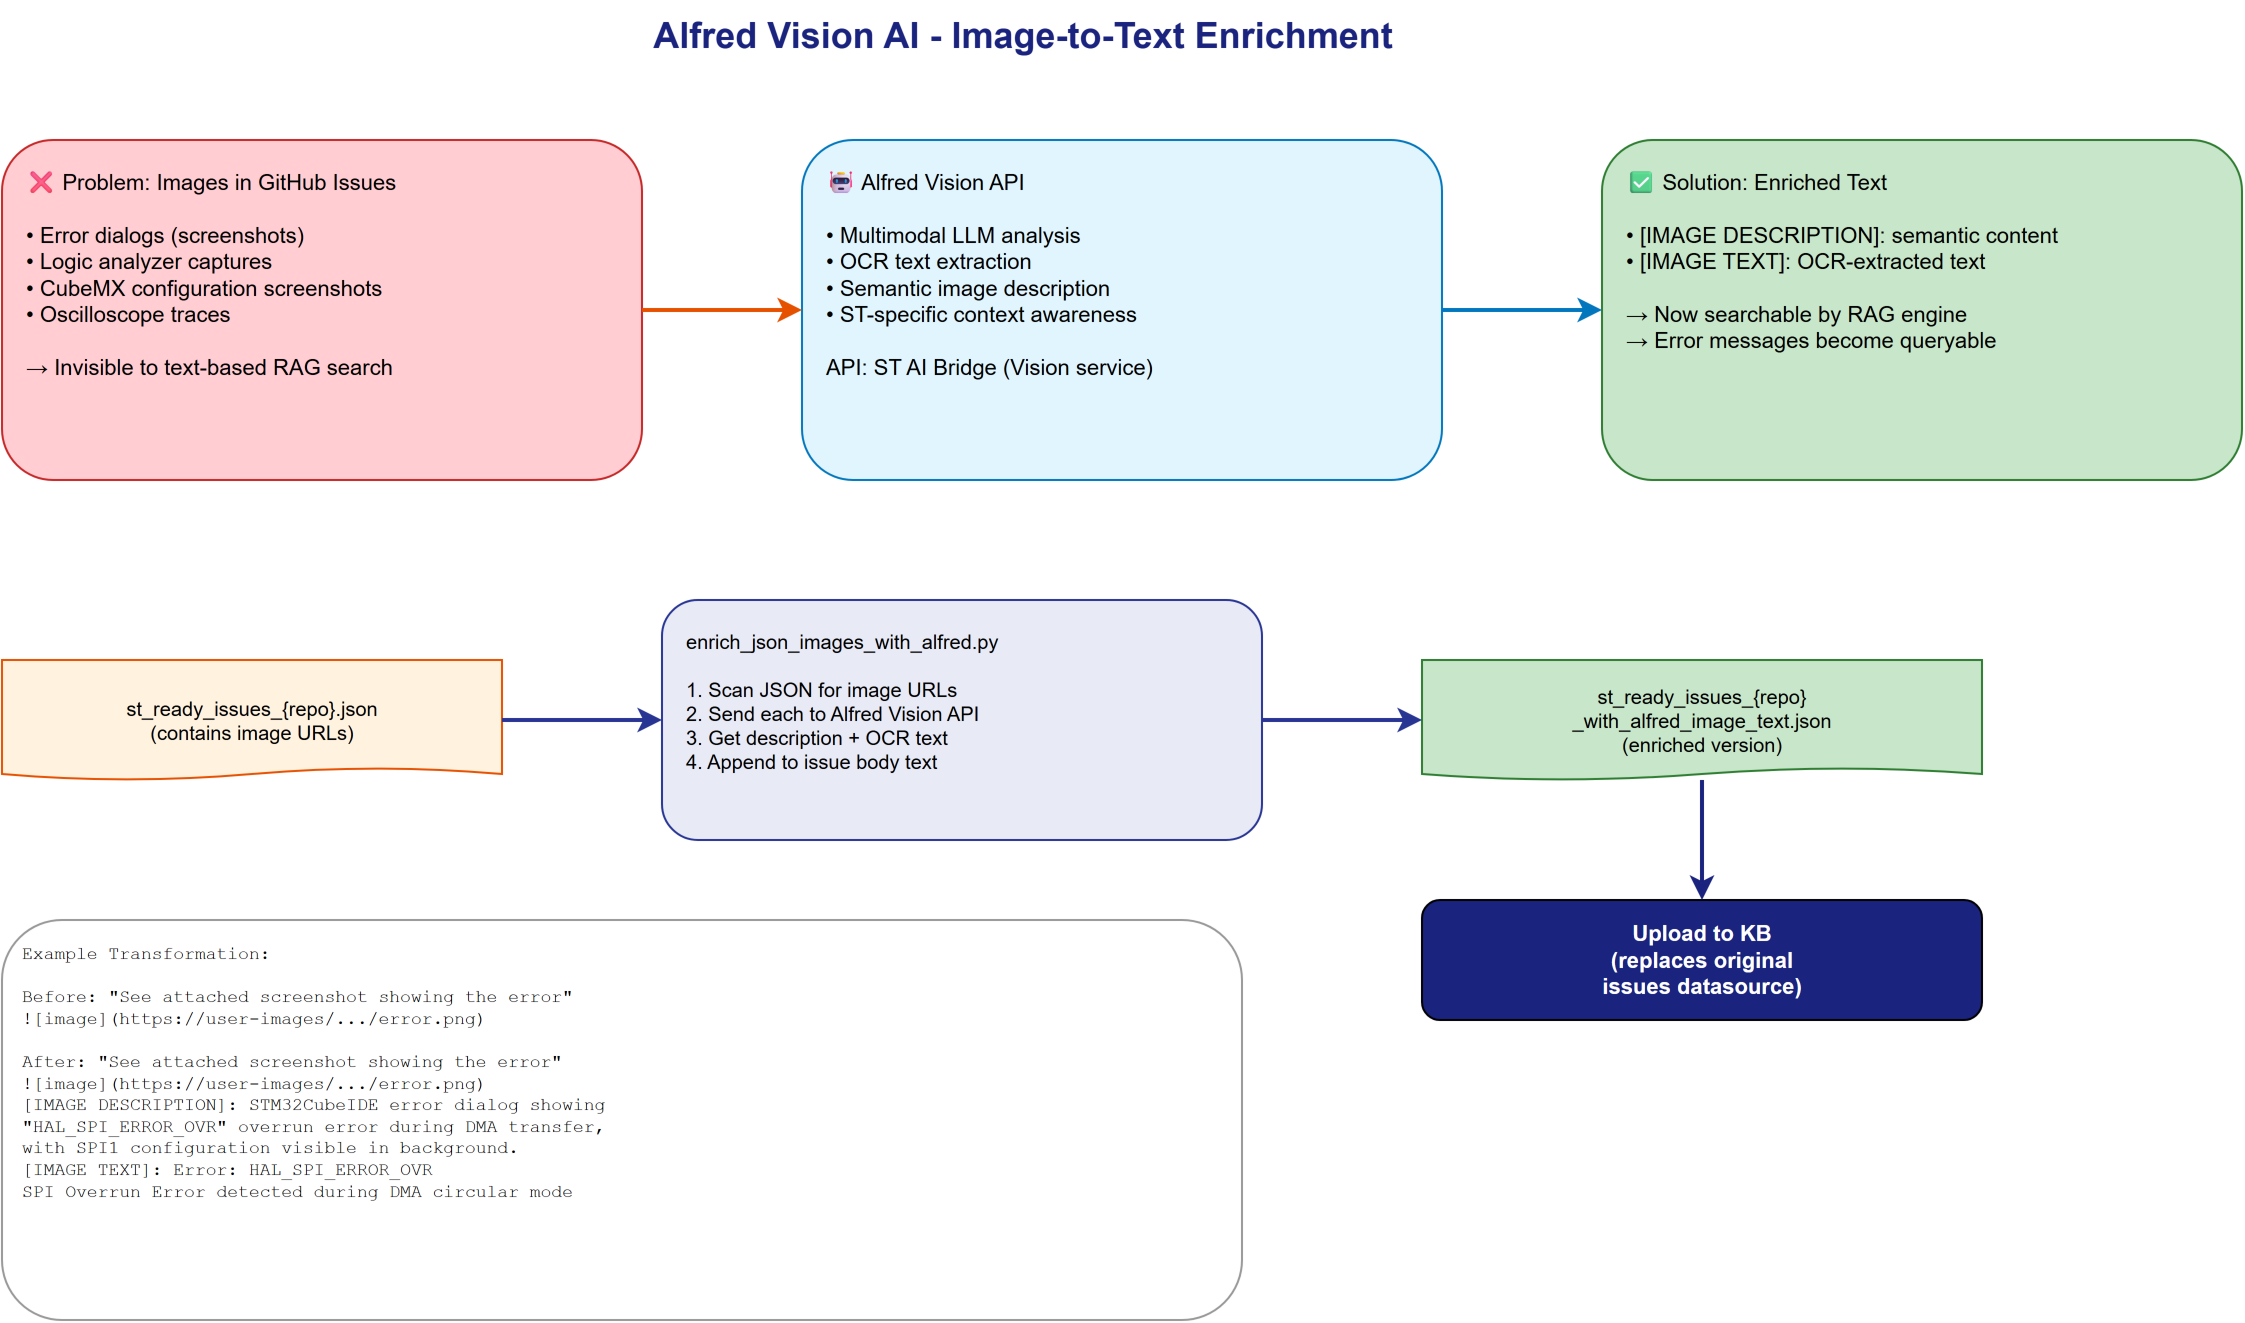
\includegraphics[width=\textwidth]{05_alfred_vision_integration.png}
  \caption{Alfred Vision AI integration: image URL extraction, API call, text injection}
  \label{fig:alfred-integration}
\end{figure}

\begin{lstlisting}[language=bash]
python pipeline_Automation/enrich_json_images_with_alfred.py \
  --input "datasets/.../st_ready_issues_stm32cubef4.json" \
  --persona "st_copilot" --strip-analyses
\end{lstlisting}

Output: \texttt{st\_ready\_issues\_\{repo\}\_with\_alfred\_image\_text.json}

Each image URL in issue text gets appended fields:
\begin{itemize}
  \item \texttt{[IMAGE DESCRIPTION]} --- Semantic description of the image content
  \item \texttt{[IMAGE TEXT]} --- OCR-extracted text from the image
\end{itemize}

%% ============================================================
\chapter{Persona Configuration}
%% ============================================================

\section{Recommended Settings}

\begin{longtable}{p{5cm}p{8cm}}
\toprule
\textbf{Parameter} & \textbf{Value} \\
\midrule
Tool Name & ST-GitHub-Analyzer-Unstructured \\
Search Type & Hybrid (Semantic + Full-text) \\
Semantic Threshold & 0.55 \\
Semantic Max Doc Count & 20 \\
Full-text Max Doc Count & 12 \\
\bottomrule
\end{longtable}

\section{System Prompt}

The persona system prompt follows a 4-case answer strategy:
\begin{enumerate}
  \item Direct KB match → cite source
  \item Partial match → diagnosis + candidate workaround + validation steps
  \item General configuration question → direct technical explanation
  \item No match → actionable next step (never only ``I don't know'')
\end{enumerate}

%% ============================================================
\chapter{Automation \& Operations}
%% ============================================================

\section{Full Workflow Execution}

\begin{figure}[H]
  \centering
  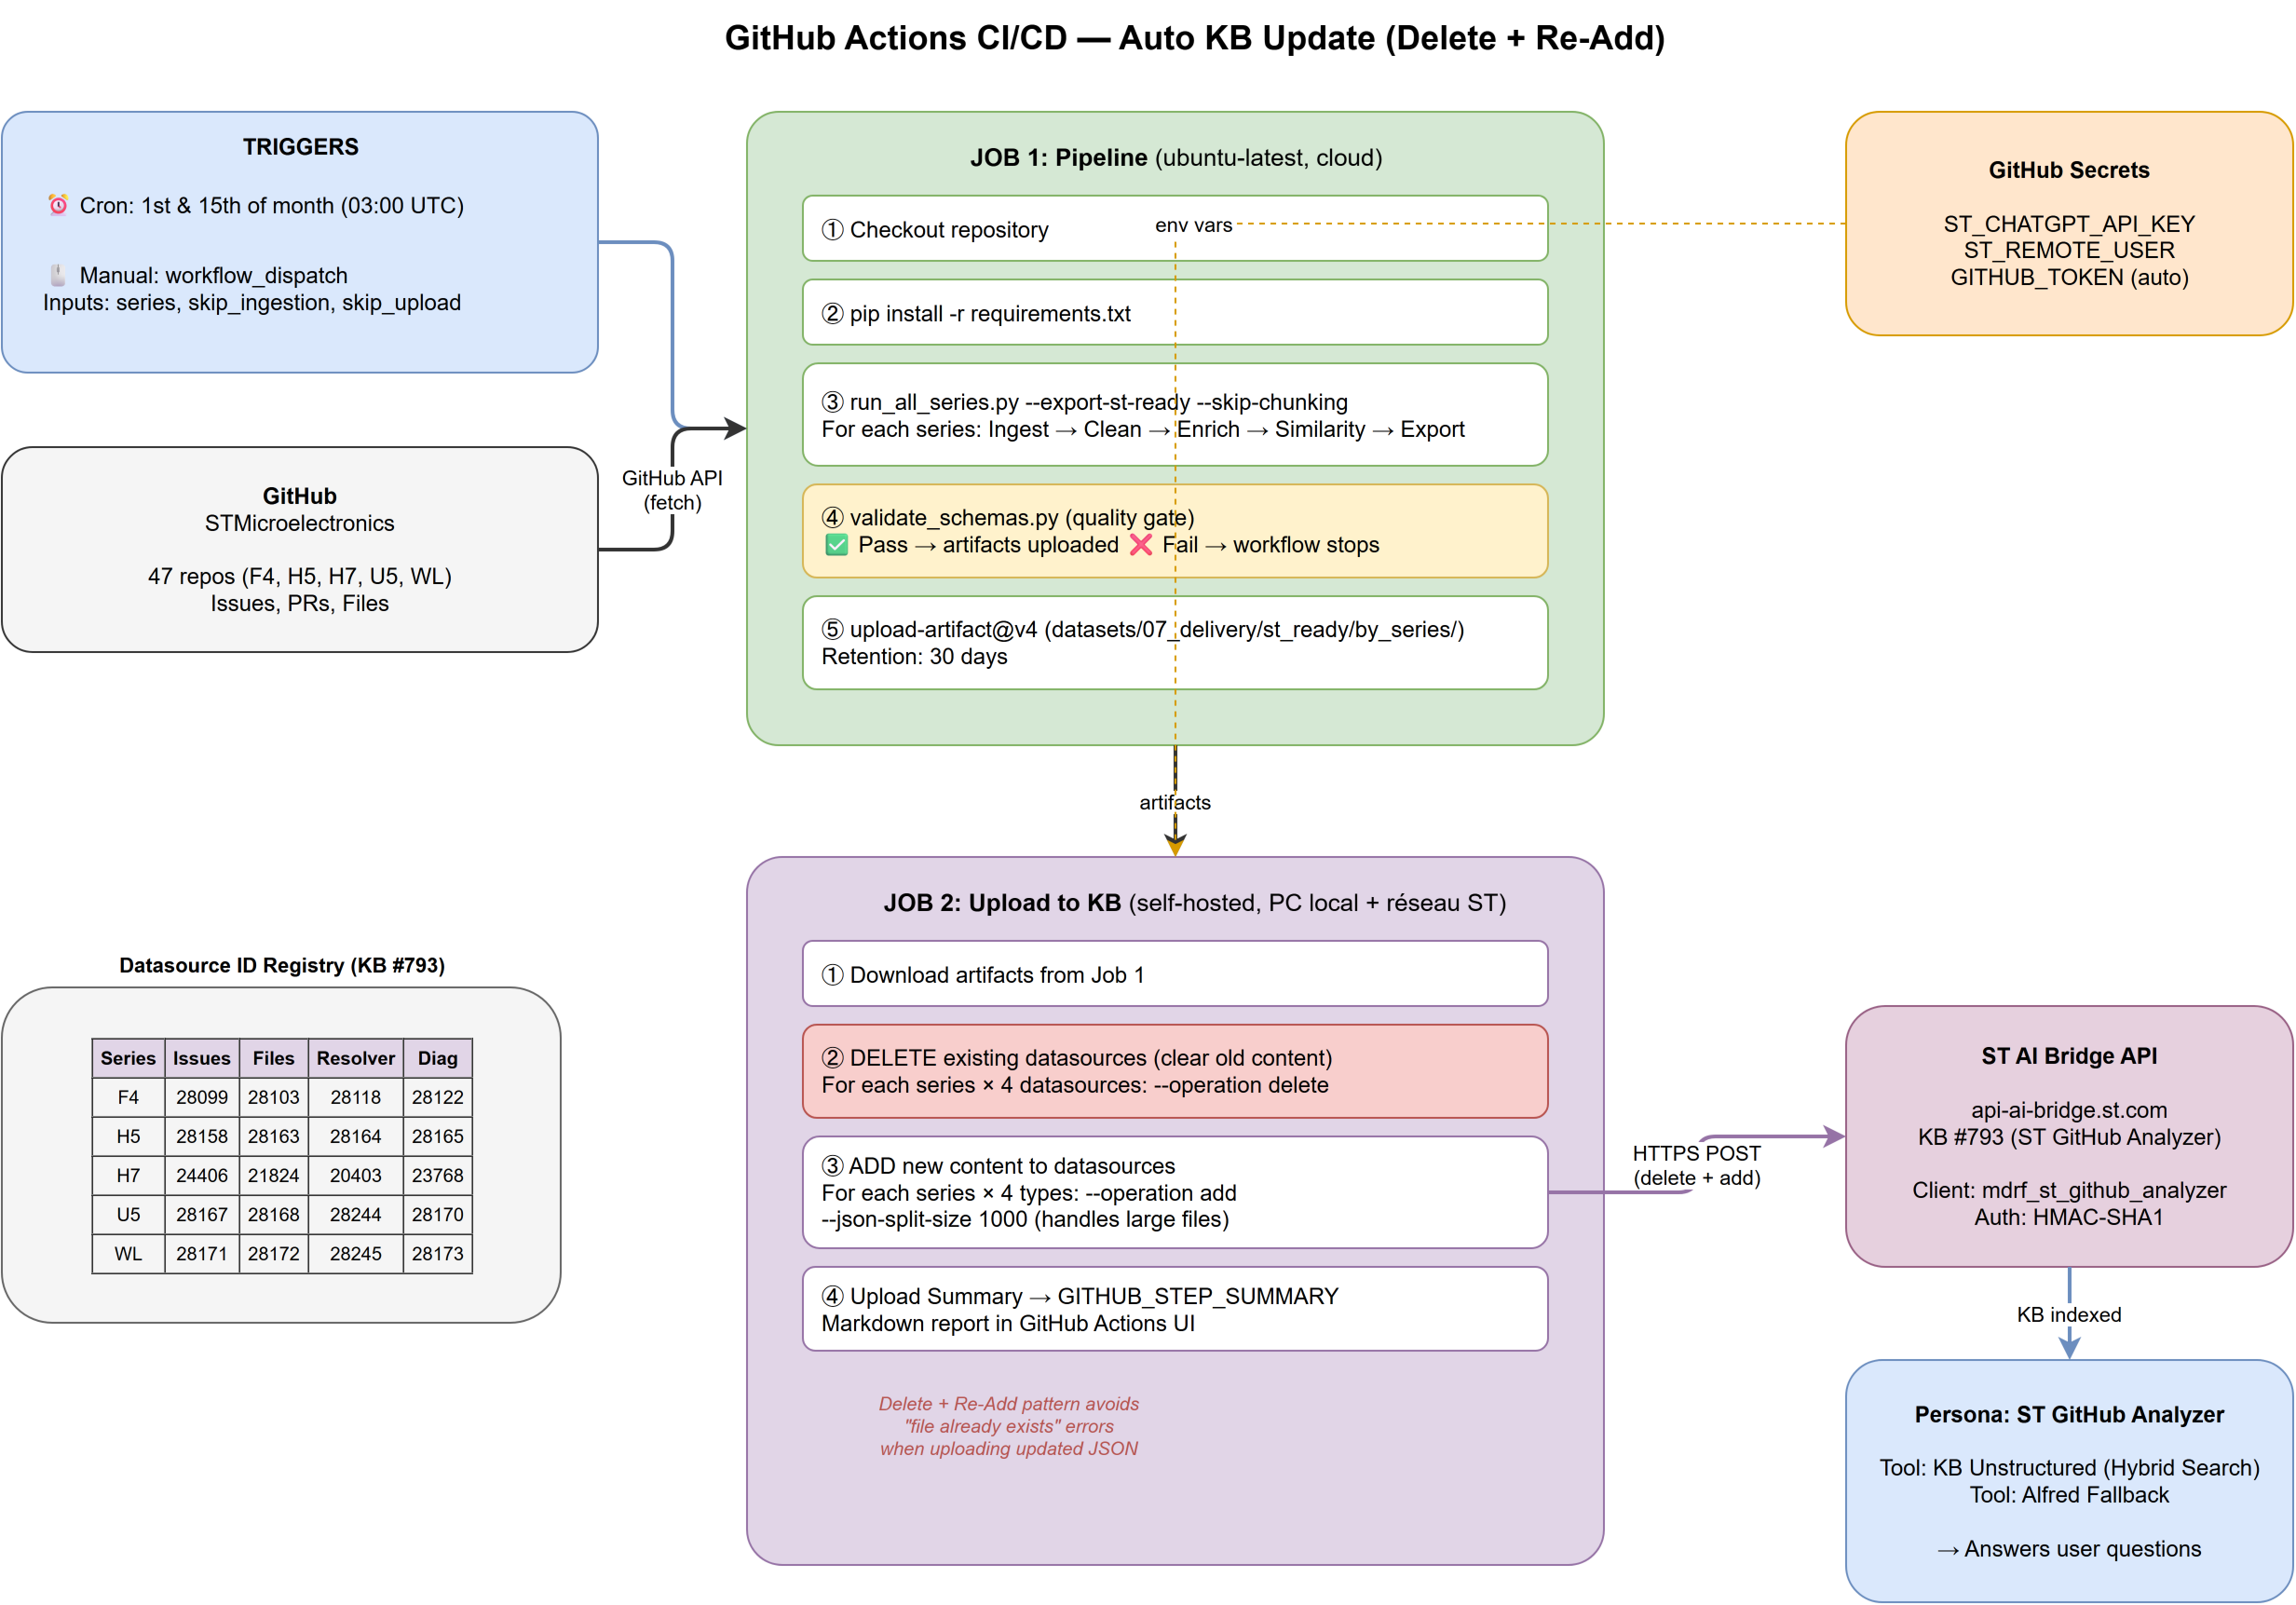
\includegraphics[width=\textwidth]{06_cicd_automation.png}
  \caption{CI/CD automation: GitHub Actions workflow with delete+add upload pattern}
  \label{fig:cicd-automation}
\end{figure}

\begin{figure}[H]
  \centering
  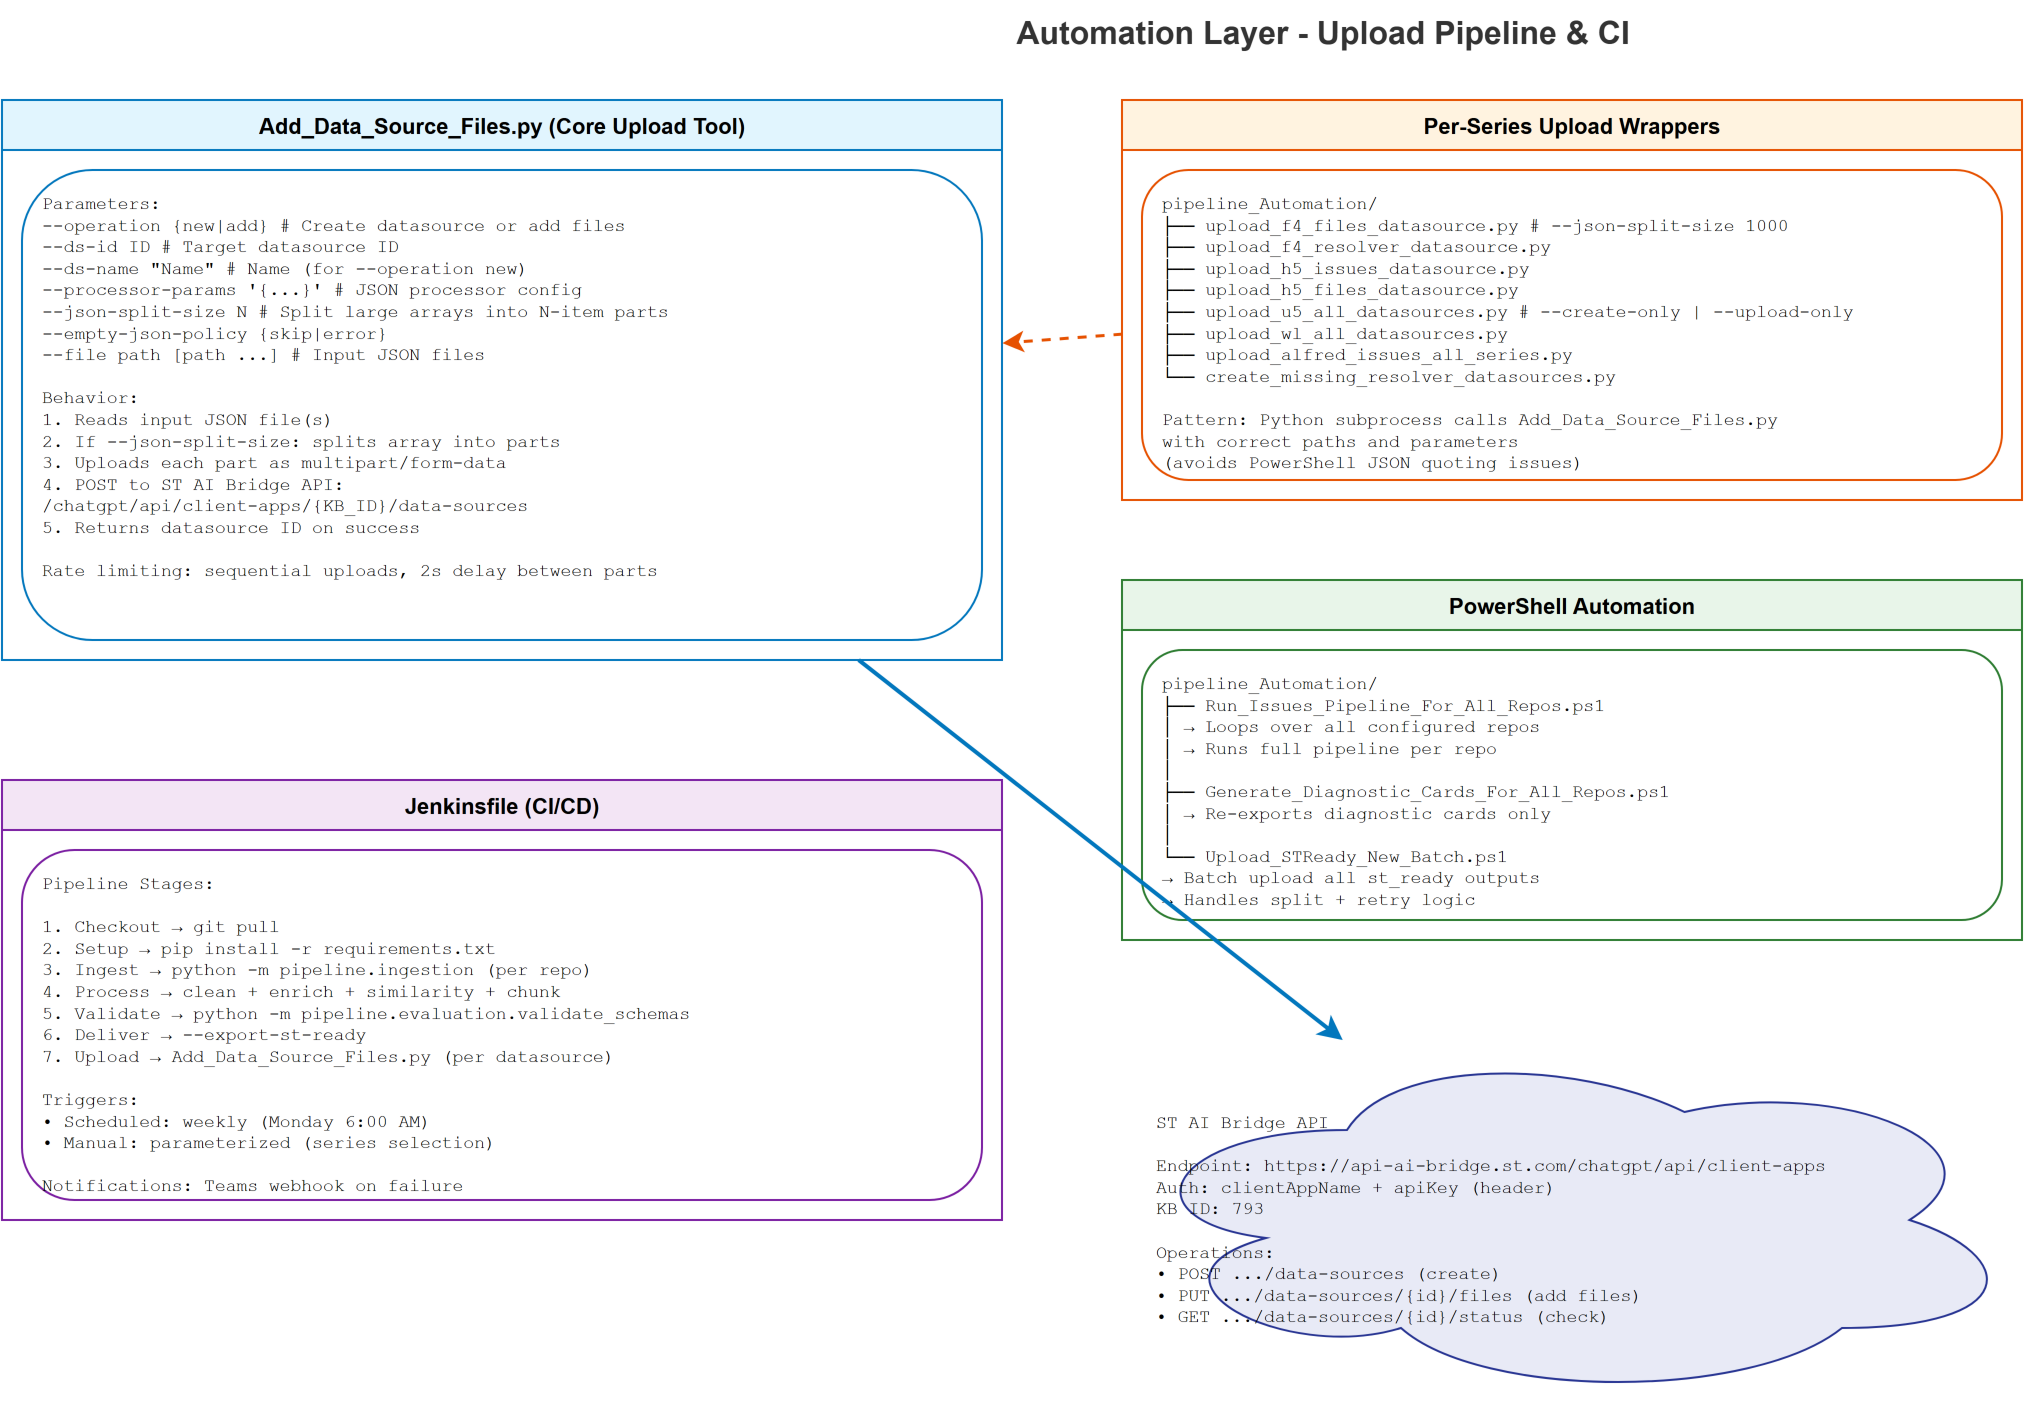
\includegraphics[width=0.9\textwidth]{06_automation_ci_upload.png}
  \caption{Automation architecture: scheduled triggers, validation gates, and upload}
  \label{fig:automation-upload}
\end{figure}

\begin{lstlisting}[language=bash]
# Standard run
python -m pipeline.run_full_workflow

# With delivery export
python -m pipeline.run_full_workflow --export-st-ready

# Skip ingestion (reprocess from existing raw data)
python -m pipeline.run_full_workflow --skip-ingestion --continue-on-error
\end{lstlisting}

\section{Multi-Series Automation}

\begin{lstlisting}[language=bash]
# Run all series sequentially
python -m pipeline_Automation.run_all_series

# Re-export delivery only (no re-ingestion)
python -m pipeline_Automation.reexport_delivery --series f4 --continue-on-error
\end{lstlisting}

\section{Upload Scripts}

Per-series upload scripts handle datasource creation and file upload:
\begin{itemize}
  \item \texttt{upload\_f4\_files\_datasource.py}, \texttt{upload\_f4\_resolver\_datasource.py}, etc.
  \item \texttt{upload\_u5\_all\_datasources.py} --- Creates + uploads all 4 types
  \item \texttt{upload\_alfred\_issues\_all\_series.py} --- Uploads Alfred-enriched versions
\end{itemize}

\section{Fully Automated KB Update (End-to-End)}

The script \texttt{pipeline\_Automation/workflow/Run\_Full\_Auto\_Update\_KB.ps1} chains \textbf{all stages} in a single command:

\begin{lstlisting}[language=bash]
# Full auto-update: ingest + preprocess + export + validate + upload
.\pipeline_Automation\workflow\Run_Full_Auto_Update_KB.ps1 `
    -RemoteUser "abir.gharbi@st.com" `
    -Series f4,h5,h7,u5,wl

# Re-process only (skip GitHub fetch, keep raw data)
.\pipeline_Automation\workflow\Run_Full_Auto_Update_KB.ps1 `
    -RemoteUser "abir.gharbi@st.com" `
    -SkipIngestion

# Pipeline only, no KB upload (dry-run)
.\pipeline_Automation\workflow\Run_Full_Auto_Update_KB.ps1 `
    -SkipUpload -Series h7
\end{lstlisting}

\subsection{What the Script Does}

\begin{enumerate}
  \item Runs \texttt{run\_all\_series.py} with \texttt{--export-st-ready} for each selected MCU series
  \item Validates all outputs with \texttt{validate\_schemas}
  \item \textbf{Blocks upload if validation fails} (safety gate)
  \item Uploads each artifact type to its registered datasource ID in KB \#793
  \item Writes a timestamped log to \texttt{logs/auto\_update\_kb\_*.log}
\end{enumerate}

\subsection{Scheduling for Always-Fresh KB}

\textbf{Note:} Local chunking is skipped (\texttt{--skip-chunking}) because the ST ChatGPT platform handles document chunking internally at upload time.

\begin{longtable}{p{4cm}p{9cm}}
\toprule
\textbf{Method} & \textbf{Setup} \\
\midrule
GitHub Actions (recommended) & Workflow file \texttt{.github/workflows/auto\_update\_kb.yml} runs automatically every 2 weeks (1st and 15th of each month). Fully cloud-based --- no local machine needed. \\
Local (fallback) & Windows Task Scheduler running \texttt{Run\_Full\_Auto\_Update\_KB.ps1} every 2 weeks. Requires machine to be powered on. \\
\bottomrule
\end{longtable}

\subsection{GitHub Actions Cloud Automation (Recommended)}

The workflow \texttt{.github/workflows/auto\_update\_kb.yml} provides fully automated cloud execution:

\begin{itemize}
  \item \textbf{Trigger}: Bi-weekly cron (\texttt{0 3 1,15 * *}) + manual dispatch
  \item \textbf{Steps}: Ingest $\to$ Preprocess (no chunking) $\to$ Export $\to$ Validate $\to$ Upload $\to$ Archive
  \item \textbf{Secrets required}: \texttt{ST\_CHATGPT\_API\_KEY}, \texttt{ST\_REMOTE\_USER}, \texttt{GITHUB\_TOKEN}
  \item \textbf{No local machine needed}: Runs entirely on GitHub-hosted runners
  \item \textbf{Manual override}: Can be triggered on-demand via ``Run workflow'' button with custom series selection
\end{itemize}

To set up:
\begin{enumerate}
  \item Go to repository Settings $\to$ Secrets and variables $\to$ Actions
  \item Add secret \texttt{ST\_CHATGPT\_API\_KEY} with your ST AI Bridge API key
  \item Add secret \texttt{ST\_REMOTE\_USER} with your email (e.g. \texttt{abir.gharbi@st.com})
  \item Push the \texttt{.github/workflows/auto\_update\_kb.yml} file to the main branch
  \item The workflow will trigger automatically on the 1st and 15th of each month
\end{enumerate}

\subsection{Recommended Frequency}

\begin{itemize}
  \item \textbf{Weekly}: Catches new issues and community activity
  \item \textbf{On firmware release}: Run immediately after a new CubeF4/H7/etc. version is tagged
  \item \textbf{On-demand}: Before demos, evaluations, or after pipeline code changes
\end{itemize}

\subsection{Safety Guarantees}

\begin{itemize}
  \item Schema validation gate prevents corrupted data from reaching the KB
  \item \texttt{kb-datasource-add} replaces existing content (not append), so no duplicates
  \item Summary JSON files are generated for traceability (count verification)
  \item Logs capture every step for post-mortem analysis
  \item \texttt{--ContinueOnError} allows partial series to complete even if one fails
\end{itemize}

%% ============================================================
\chapter{Quality Assurance}
%% ============================================================

\section{Test Suite}

\begin{figure}[H]
  \centering
  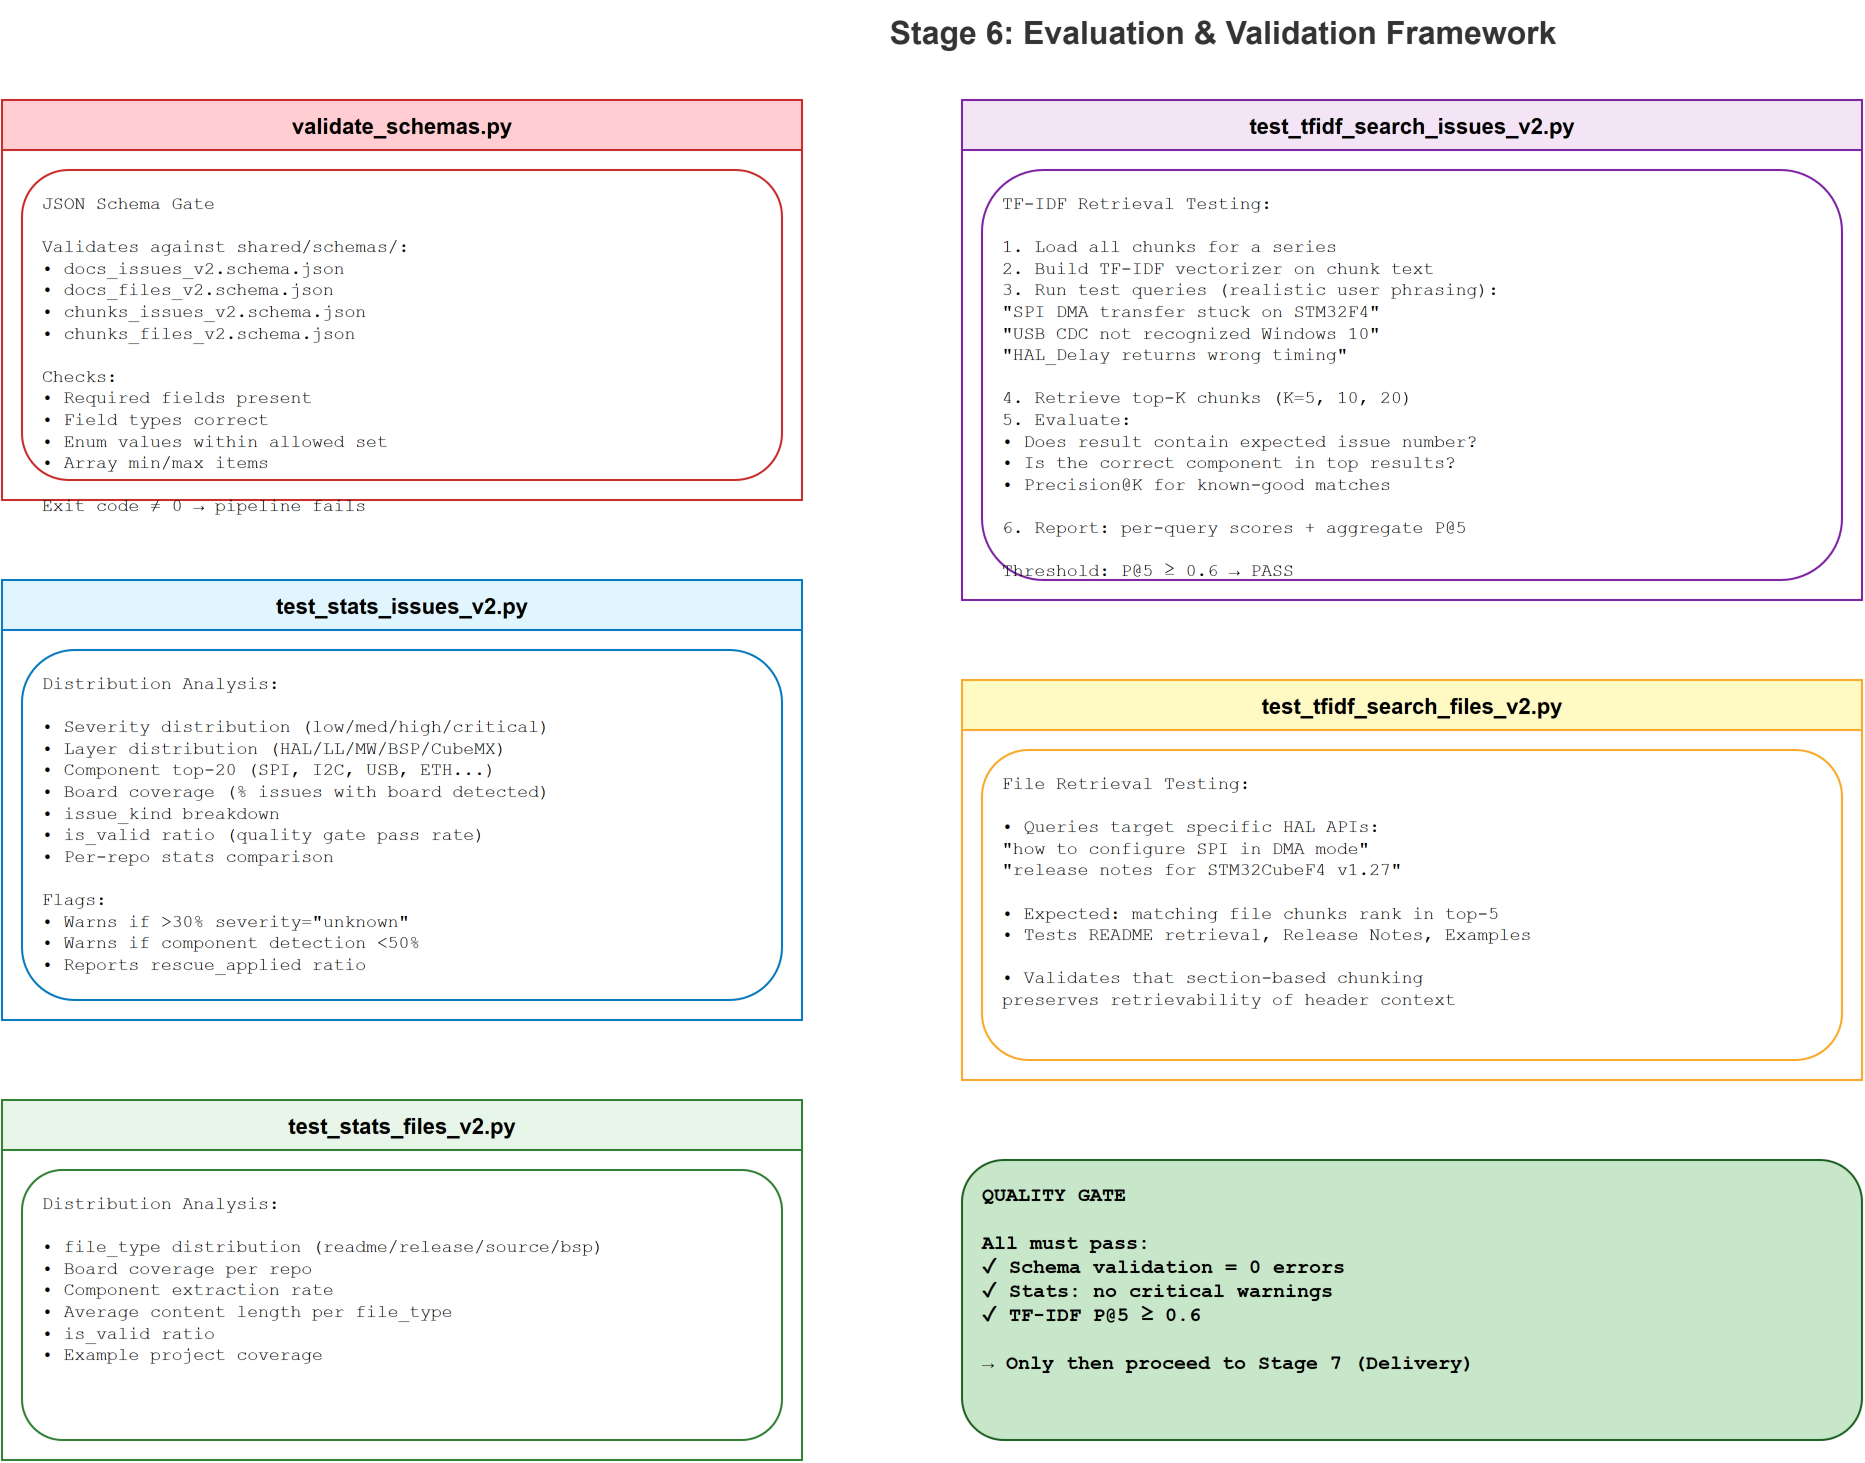
\includegraphics[width=0.9\textwidth]{05_evaluation_validation.png}
  \caption{Evaluation and validation pipeline: stats, TF-IDF tests, schema gates}
  \label{fig:evaluation-validation}
\end{figure}

50-question test suite (\texttt{all\_series\_test\_suite\_50q\_v2.csv}):
\begin{itemize}
  \item 13 questions STM32F4
  \item 12 questions STM32H5
  \item 13 questions STM32U5
  \item 12 questions STM32WL
\end{itemize}

Questions are written in realistic customer voice with symptoms, board context, and expected technical anchors.

\section{Schema Validation}

JSON schemas under \texttt{shared/schemas/} enforce structural contracts:
\begin{itemize}
  \item \texttt{docs\_issues\_v2.schema.json}
  \item \texttt{docs\_files\_v2.schema.json}
  \item \texttt{chunks\_issues\_v2.schema.json}
  \item \texttt{chunks\_files\_v2.schema.json}
\end{itemize}

Run: \texttt{python -m pipeline.evaluation.validate\_schemas}

%% ============================================================
\chapter{ST ChatGPT Platform --- Usage Guide}
%% ============================================================

\section{Platform Overview}

The ST ChatGPT platform (\texttt{https://stchatgpt.st.com}) is ST's internal deployment of Azure OpenAI, extended with:
\begin{itemize}
  \item \textbf{Personas} --- Custom AI agents with dedicated knowledge bases and system prompts
  \item \textbf{Knowledge Bases (KB)} --- Uploaded document collections enabling RAG retrieval
  \item \textbf{Tools} --- Search tools (Hybrid, Semantic, Full-text) connecting the LLM to KB content
  \item \textbf{AI Bridge API} --- REST API for programmatic KB management and datasource uploads
\end{itemize}

\section{How the Workflow Operates End-to-End}

\begin{enumerate}
  \item \textbf{Data Ingestion}: GitHub issues, PRs, commits, and file content are fetched via GitHub API and local repository clones.
  \item \textbf{Preprocessing}: Raw data is cleaned, enriched with heuristic NLP classification (layer, component, severity, board), and cross-linked via TF-IDF similarity.
  \item \textbf{Chunking}: Documents are split into retrieval-optimal chunks (max 512 tokens, 50-token overlap).
  \item \textbf{ST-Ready Export}: Four delivery artifact types are generated as JSON (issues, files, resolver cases, diagnostic cards).
  \item \textbf{KB Upload}: JSON artifacts are uploaded to KB \#793 via the AI Bridge API, creating indexed datasources.
  \item \textbf{Persona Answers}: When a user asks a question, the persona searches the KB, retrieves relevant chunks, and generates a structured answer citing sources.
\end{enumerate}

\begin{verbatim}
User Question
  -> Persona System Prompt (answer strategy)
    -> Tool: ST-GitHub-Analyzer-Unstructured (Hybrid Search)
      -> KB #793 (Semantic + Full-text index)
        -> Retrieved chunks (issues, files, resolver, diagnostic)
          -> LLM generates structured answer with citations
\end{verbatim}

\section{Knowledge Base Content Structure}

KB \#793 contains 4 datasource types per MCU series (F4, H5, H7, U5, WL):

\begin{longtable}{p{4cm}p{4cm}p{5cm}}
\toprule
\textbf{Datasource Type} & \textbf{File Pattern} & \textbf{Content} \\
\midrule
Issues & \texttt{st\_ready\_issues\_*.json} & Structured issue cards with metadata, symptoms, root cause, fix \\
Files & \texttt{st\_ready\_files\_*.json} & Technical documentation from HAL drivers, BSP, CMSIS, examples \\
Resolver Cases & \texttt{st\_ready\_resolver\_*.json} & Issue$\to$PR$\to$Commit fix chains with traceability \\
Diagnostic Cards & \texttt{st\_ready\_diagnostic\_*.json} & Structured fault analysis with hypotheses, checks, workarounds \\
\bottomrule
\end{longtable}

\subsection{File Organization in KB}

Each series groups its main repo and sub-repositories (drivers, BSP, CMSIS):

\begin{lstlisting}[language=bash]
by_series/
|-- stm32cubef4/
|   |-- issues_json/          # Main repo issues
|   |-- files_json/           # Main repo files
|   |-- resolver_cases_json/  # Fix chains
|   |-- diagnostic_cards_json/# Diagnostic analysis
|   +-- drivers/              # Sub-repos (HAL, BSP, CMSIS)
|       |-- stm32f4xx-hal-driver/
|       |-- cmsis_device_f4/
|       +-- stm32f4xx-nucleo-bsp/
|-- stm32cubeh7/
|-- stm32cubeh5/
|-- stm32cubeu5/
+-- stm32cubewl/
\end{lstlisting}

\subsection{What Each Datasource Enables}

\begin{itemize}
  \item \textbf{Issues}: Answers questions about known bugs, workarounds, and community-reported problems
  \item \textbf{Files}: Answers questions about HAL/LL API usage, driver configuration, BSP initialization, release notes
  \item \textbf{Resolver Cases}: Enables tracing from symptom to exact commit/PR fix
  \item \textbf{Diagnostic Cards}: Provides structured troubleshooting flow (facts $\to$ hypotheses $\to$ checks $\to$ workaround)
\end{itemize}

%% ============================================================
\chapter{Persona Configuration --- Best Practices}
%% ============================================================

\section{Recommended Persona Settings}

\begin{longtable}{p{5.5cm}p{3cm}p{5cm}}
\toprule
\textbf{Parameter} & \textbf{Recommended} & \textbf{Rationale} \\
\midrule
Tool Name & \footnotesize ST-GitHub-Analyzer-Unstructured & Hybrid search tool \\
Search Type & Hybrid & Combines semantic understanding + exact keyword matching \\
Semantic Threshold & 0.55 & Below 0.5: too much noise; above 0.65: misses partial matches \\
Semantic Max Doc Count & 20 & Balances coverage with context window limits \\
Full-text Max Doc Count & 12 & Ensures keyword-heavy queries (API names, error codes) find exact matches \\
Temperature & 0.2--0.3 & Low = factual, deterministic answers \\
Max Tokens (response) & 2000--3000 & Enough for structured diagnosis; not wasteful \\
\bottomrule
\end{longtable}

\section{System Prompt Design}

The persona system prompt must enforce:

\begin{enumerate}
  \item \textbf{4-case answer strategy}:
  \begin{itemize}
    \item Direct KB match $\to$ cite source with GitHub link
    \item Partial match $\to$ diagnosis + candidate workaround + validation steps
    \item General configuration question $\to$ direct technical explanation
    \item No match $\to$ actionable next step (never only ``I don't know'')
  \end{itemize}

  \item \textbf{Mandatory clarification questions}: The persona must always ask follow-up questions (exact MCU part, board, firmware version, reproduction steps) before providing a definitive fix.

  \item \textbf{Citation format}: Every answer must include the source GitHub URL and issue/file reference.

  \item \textbf{Scope declaration}: The prompt must declare which MCU series are covered and redirect gracefully for unsupported series.
\end{enumerate}

\section{What Works Well (Proven Patterns)}

\begin{itemize}
  \item \textbf{API-name anchoring}: Questions mentioning exact HAL/LL function names (e.g., \texttt{HAL\_SPI\_Transmit\_DMA}) retrieve with high precision because diagnostic cards include \texttt{query\_aliases} and \texttt{api\_family\_tags}.
  \item \textbf{Board + component queries}: ``NUCLEO-F446RE SPI timeout'' retrieves accurately thanks to enriched metadata fields.
  \item \textbf{Symptom-based retrieval}: Diagnostic cards contain \texttt{symptom\_summary} and \texttt{technical\_pattern\_tags} enabling natural-language symptom matching.
  \item \textbf{Version-specific questions}: \texttt{version\_tags} enable retrieval for upgrade/regression scenarios.
\end{itemize}

\section{Known Limitations}

\begin{longtable}{p{5cm}p{8cm}}
\toprule
\textbf{Limitation} & \textbf{Impact \& Mitigation} \\
\midrule
Context window saturation & With 20 semantic + 12 full-text docs, complex queries may hit token limits. Mitigation: chunking keeps individual docs small ($\leq$512 tokens). \\
Image content opacity & Screenshots in issues are opaque to text search. Mitigation: Alfred Vision AI enrichment converts images to text descriptions. \\
Stale data & KB content reflects the last pipeline run. Mitigation: schedule periodic re-runs (weekly or after major Cube releases). \\
Cross-series confusion & Questions without explicit series may retrieve answers from wrong MCU family. Mitigation: system prompt enforces clarification questions. \\
Low-signal issues & Some GitHub issues contain only conversational noise (``thank you'', ``+1''). Mitigation: \texttt{is\_valid} filter and \texttt{rescue\_applied} heuristic. \\
Large file splits & Files $>$10MB require splitting into parts, which may fragment context. Mitigation: \texttt{--json-split-size 1000} keeps parts manageable. \\
\bottomrule
\end{longtable}

\section{Anti-Patterns to Avoid}

\begin{itemize}
  \item \textbf{DO NOT} set semantic threshold below 0.4 --- retrieves too much irrelevant content
  \item \textbf{DO NOT} disable full-text search --- API names and error codes need exact matching
  \item \textbf{DO NOT} upload raw GitHub JSON without preprocessing --- the persona cannot parse unstructured API responses
  \item \textbf{DO NOT} skip diagnostic cards --- they are the primary structured troubleshooting source
  \item \textbf{DO NOT} use temperature $>$ 0.5 for technical answers --- causes hallucination of non-existent fixes
  \item \textbf{DO NOT} merge all series into a single datasource --- separate datasources per series improve precision and allow targeted updates
\end{itemize}

%% ============================================================
\chapter{KB Maintenance \& Update Workflow}
%% ============================================================

\section{When to Re-run the Pipeline}

\begin{itemize}
  \item After a new STM32Cube firmware release (e.g., v1.29.0)
  \item After significant issue activity (20+ new issues since last run)
  \item After adding support for a new MCU series
  \item Before a major demo or evaluation cycle
\end{itemize}

\section{Update Procedure}

\begin{lstlisting}[language=bash]
# 1. Re-run pipeline with fresh ingestion
python -m pipeline.run_full_workflow --export-st-ready

# 2. Validate outputs
python -m pipeline.evaluation.validate_schemas

# 3. Upload new batch to KB
python pipeline_Automation/upload/Add_Data_Source_Files.py \
  --input "datasets/07_delivery/st_ready/by_series/stm32cubef4/issues_json/*.json" \
  --datasource-id 28099 --json-split-size 1000

# 4. Verify in ST ChatGPT platform
# -> Open persona -> Test a known question -> Confirm source citations
\end{lstlisting}

\section{Datasource Versioning Strategy}

\begin{itemize}
  \item Each upload \textbf{replaces} the previous datasource content (not append).
  \item Keep the previous JSON export as backup before uploading.
  \item Use \texttt{summary\_*.json} files to track counts and verify no data loss.
  \item Monitor for regressions using the 50-question test suite after each upload.
\end{itemize}

\section{Adding a New MCU Series}

\begin{enumerate}
  \item Create \texttt{shared/config/config\_\{series\}.json} with the repository list
  \item Run: \texttt{python -m pipeline.run\_full\_workflow --config config\_\{series\}.json --export-st-ready}
  \item Create 4 datasources in KB \#793 (issues, files, resolver, diagnostic)
  \item Upload the generated JSON files
  \item Add 10--15 test questions covering the new series
  \item Update the persona system prompt to declare the new series as supported
\end{enumerate}

%% ============================================================
\chapter{Evaluation \& Benchmarking Protocol}
%% ============================================================

\section{50-Question Test Suite}

The evaluation protocol uses a curated question set with:
\begin{itemize}
  \item Realistic customer voice (symptoms, not solutions)
  \item Board and version context included
  \item Expected technical anchors documented for each question
  \item Coverage across all 5 series and multiple issue types
\end{itemize}

\section{Scoring Criteria}

Each answer is scored on 4 dimensions:

\begin{longtable}{p{3.5cm}p{3cm}p{6.5cm}}
\toprule
\textbf{Dimension} & \textbf{Weight} & \textbf{Criteria} \\
\midrule
Retrieval Relevance & 30\% & Did the persona find the right KB document? \\
Technical Accuracy & 30\% & Is the answer factually correct? \\
Actionability & 25\% & Can the user act on the response without further research? \\
Citation Quality & 15\% & Are sources cited with valid GitHub URLs? \\
\bottomrule
\end{longtable}

\section{A/B Testing}

When testing configuration changes (threshold, doc count, prompt wording):
\begin{enumerate}
  \item Run the 50-question suite on configuration A (baseline)
  \item Apply the change and run on configuration B
  \item Compare scores per dimension
  \item Only deploy B if it improves retrieval relevance without degrading accuracy
\end{enumerate}

%% ============================================================
\chapter{Appendix}
%% ============================================================

\section{Diagram Index}

\subsection{Presentation Diagrams}
\begin{enumerate}
  \item \texttt{01\_pipeline\_overview.drawio} --- High-level 7-stage pipeline
  \item \texttt{02\_delivery\_kb\_upload.drawio} --- Delivery artifacts + KB upload
  \item \texttt{03\_data\_flow\_source\_to\_answer.drawio} --- End-to-end data flow
\end{enumerate}

\subsection{Technical Diagrams}
\begin{enumerate}
  \item \texttt{01\_ingestion\_detail.drawio} --- Ingestion scripts and outputs
  \item \texttt{02\_enrichment\_similarity\_detail.drawio} --- Heuristic classification
  \item \texttt{03\_delivery\_resolver\_diagnostic.drawio} --- Resolver/diagnostic generation
\end{enumerate}

\section{Environment}

\begin{itemize}
  \item Python 3.14+
  \item Virtual environment: \texttt{.venv/}
  \item Key dependencies: requests, scikit-learn (TF-IDF), openpyxl
  \item OS: Windows 11 (OneDrive workspace)
  \item IDE: VS Code with Copilot
\end{itemize}

\end{document}
